\subsection{Test Journal: Component models} \label{app:tj_0}

\textbf{Executed by: Kasper} \\
\textbf{Date: 12/5/2022}

\subsubsection*{Objective}
This test aims to document the behavior of the component models defined in \cref{sec:reformulation-of-components}.

\subsubsection*{Background}
In the plots in \cref{sec:model-verification} the states $ M_{pjj} $ and $ M_{con} $ seemed to be integrating. This indicated that the component models were not connected in an appropriate way.
Additionally in the B matrix of the linearised system, found in \cref{eq:B}, the system also showed that the compressor speed and the condenser throttle valve opening degree did not affect the states of interest, which further indicates that the non linear model could be flawed.
Before connecting all the components into one big new system, an intermediate step will be introduced. This is a verification of all of the individual component models.


\subsubsection*{Test subject}
The test subjects are the classes
\begin{itemize}
	\item boxModel
	\item compressorModel
	\item condenserModel
	\item evaporatorModel
	\item flashtankModel
	\item pjjModel
	\item valveModel
\end{itemize}
All the components are based on the models defined in \cref{sec:mod_comp_mod}. Some of them are modified with changes defined in \cref{sec:reformulation-of-components}.\\

The following components are implemented according to \cref{sec:mod_comp_mod}.
\begin{itemize}
	\item boxModel
	\item compressorModel
	\item condenserModel
	\item evaporatorModel
\end{itemize}

The following components are modified completely according to \cref{sec:reformulation-of-components}:

\begin{itemize}
	\item flashtankModel
	\item pjjModel
	\item valveModel
\end{itemize}

The aim is to test the components before more states are introduced, in order to not introduce extra complexities before a the simplest models are confirmed. This also means that the extra states in the condenser and evaporator is not tested in this test.


\subsubsection*{Equipment used}
The outputs from a simulation of "eTRU\_prototype\_2\_old\_perhabs\_with\_measurements.slx" are used as inputs for the test. The imported data can be found in "HiFi\_model\_data\_for\_component\_tests\_03.mat".
The script used for the tests are to be found in "componentModelTesting.m". with support from testinit.m.
All the files can be found in the git repository under CA8Project/Modeling/ComponentSimulation with the commit hash 25682de26edbdb141551d64b280ee66e48e26d2e.

\subsubsection*{Test setup}
The component models are compared to the HiFi simulation. This means that the measurements that are inputs to the components in the Hifi simulation model are used as inputs to the test subjects: the component models. The outputs of the test subjects are then compared with the outputs of the component models of the HiFi model.

\subsubsection*{Test procedure}
Run the script "ComponentModelTesting.m".

\clearpage
\subsubsection*{Results and Comments}

\begin{figure}[h]
	\centering
	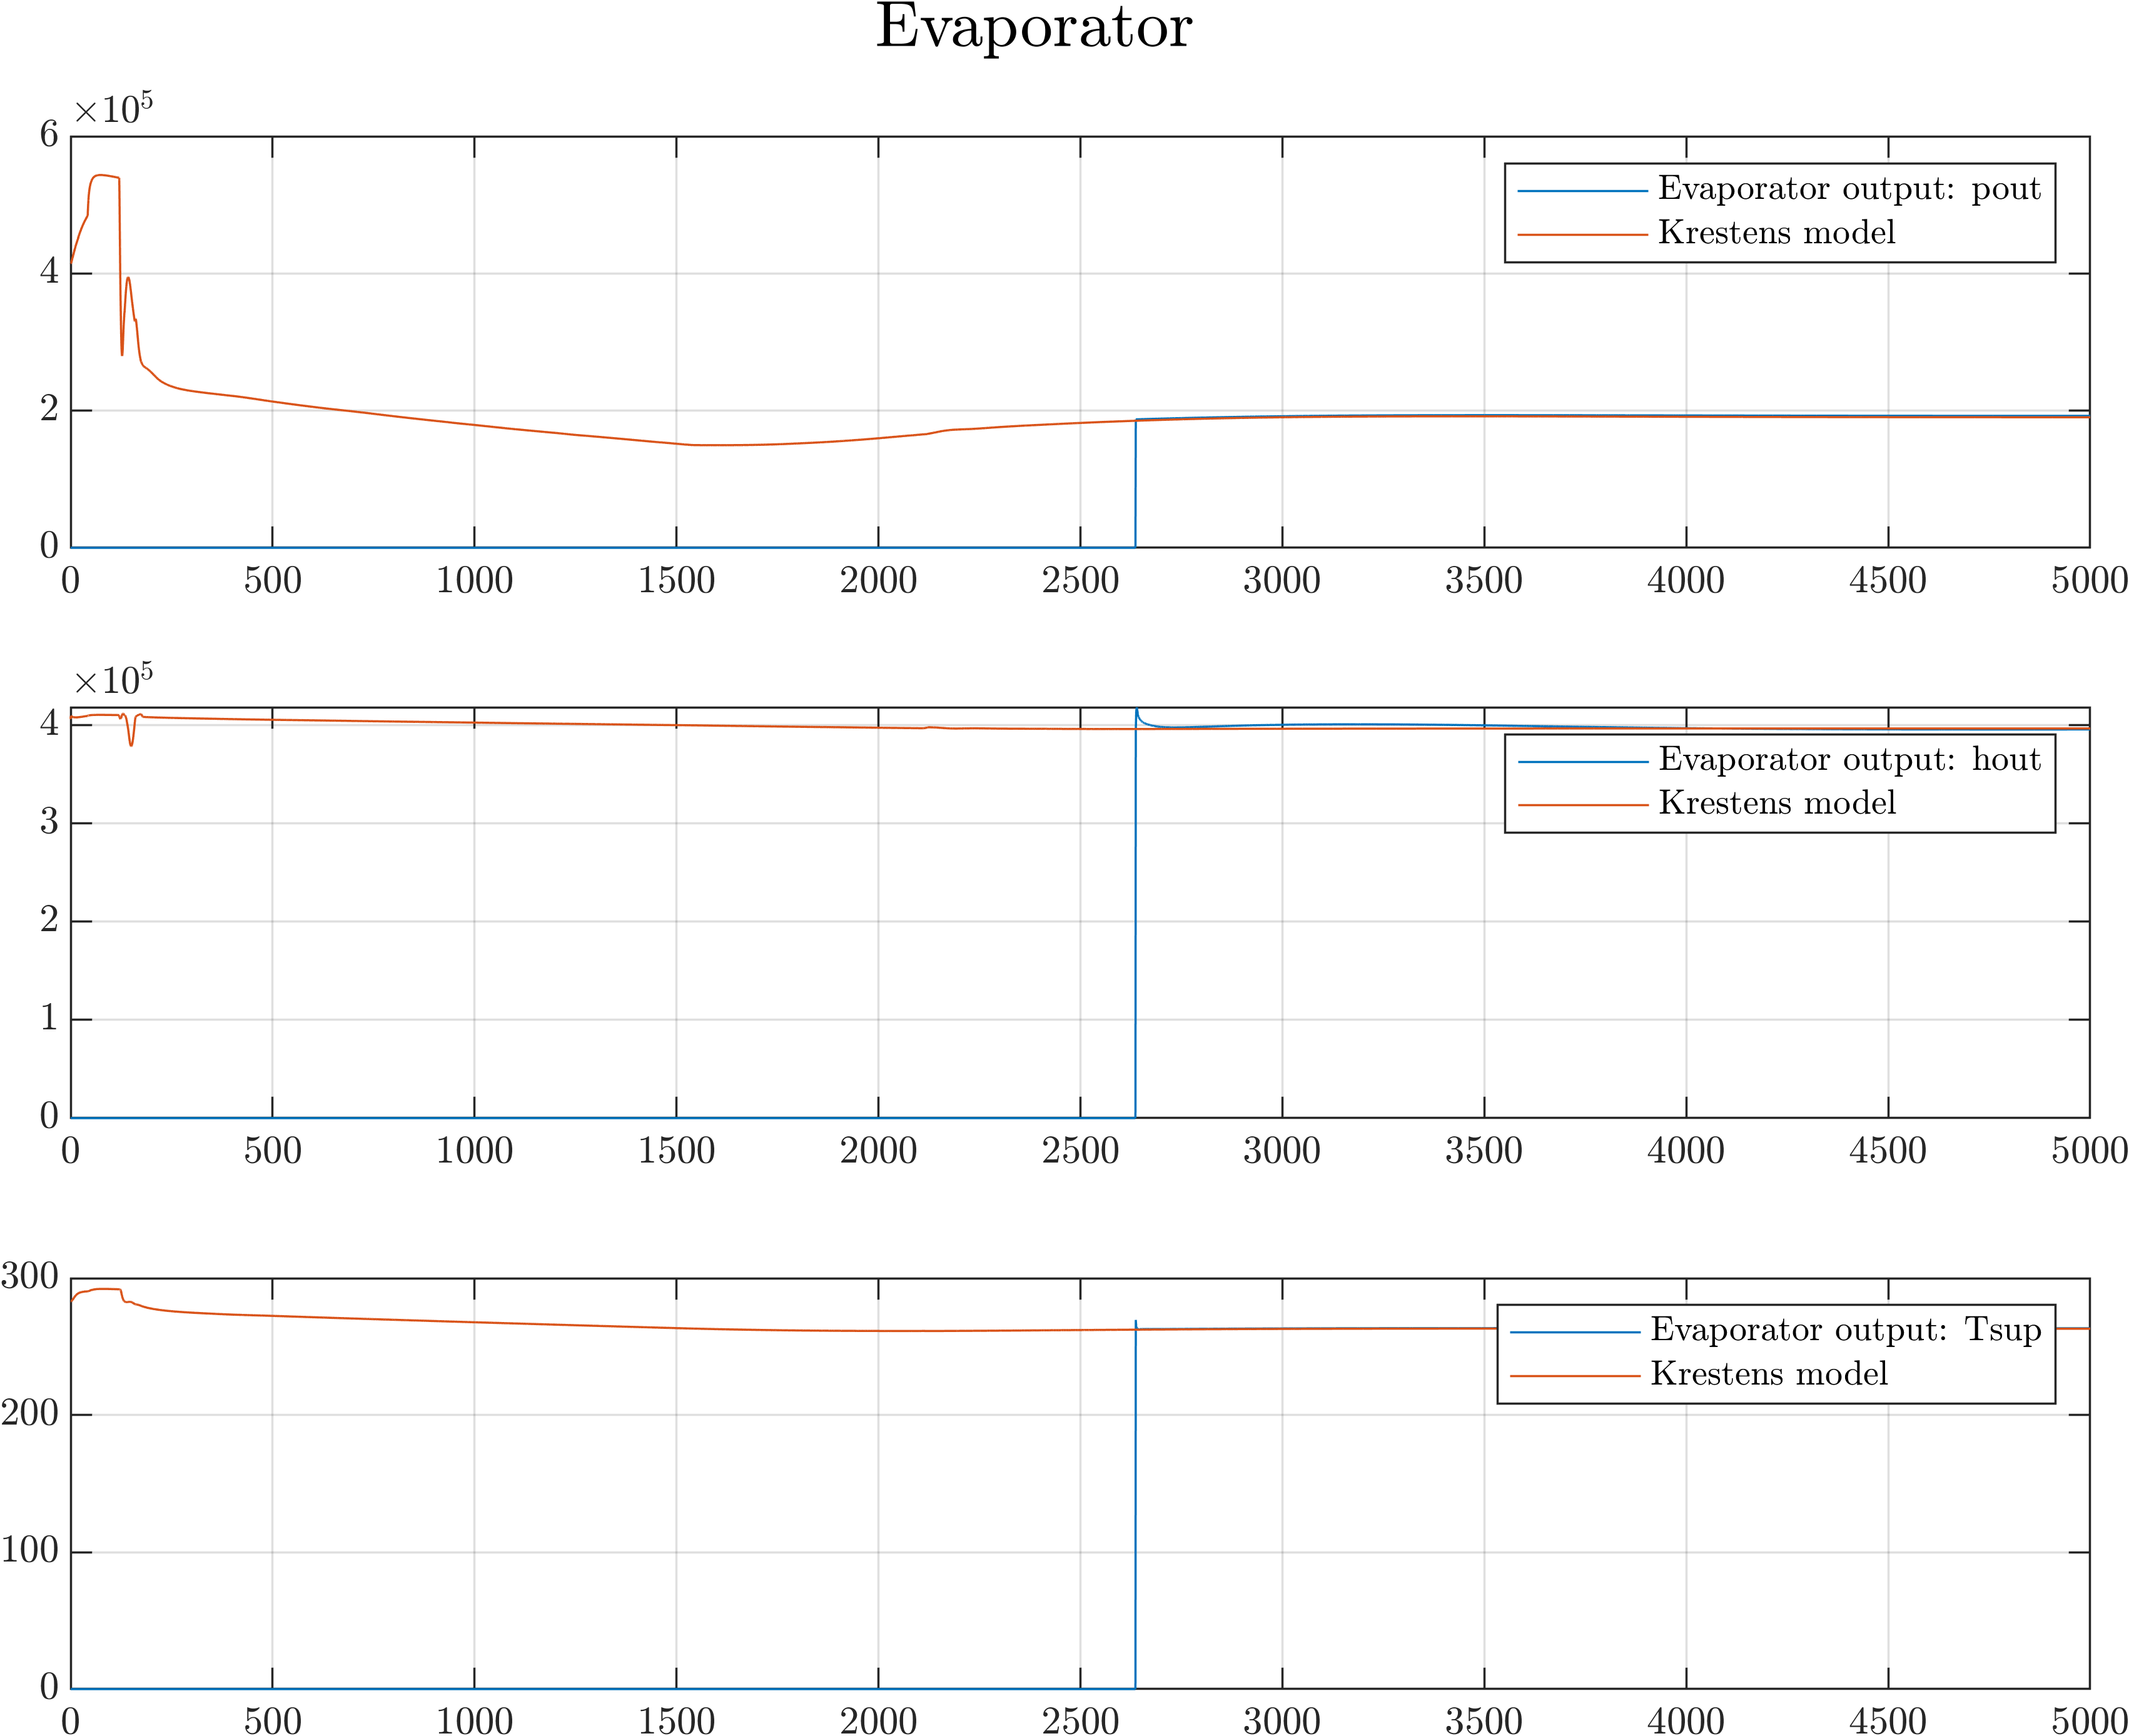
\includegraphics[width=1\textwidth]{Graphics/comp_test_com.png}
	\caption{Comparison of compressorModel outputs with HiFi component model of compressor}
	\label{fig:component_test_com}
\end{figure}
The compressorModel resembles the HiFi model (Krestens model) well. The difference is only mention-able in the transient from 500 s to 1750 s. The accuracy is considered satisfactory.
\clearpage
\begin{figure}[h]
	\centering
	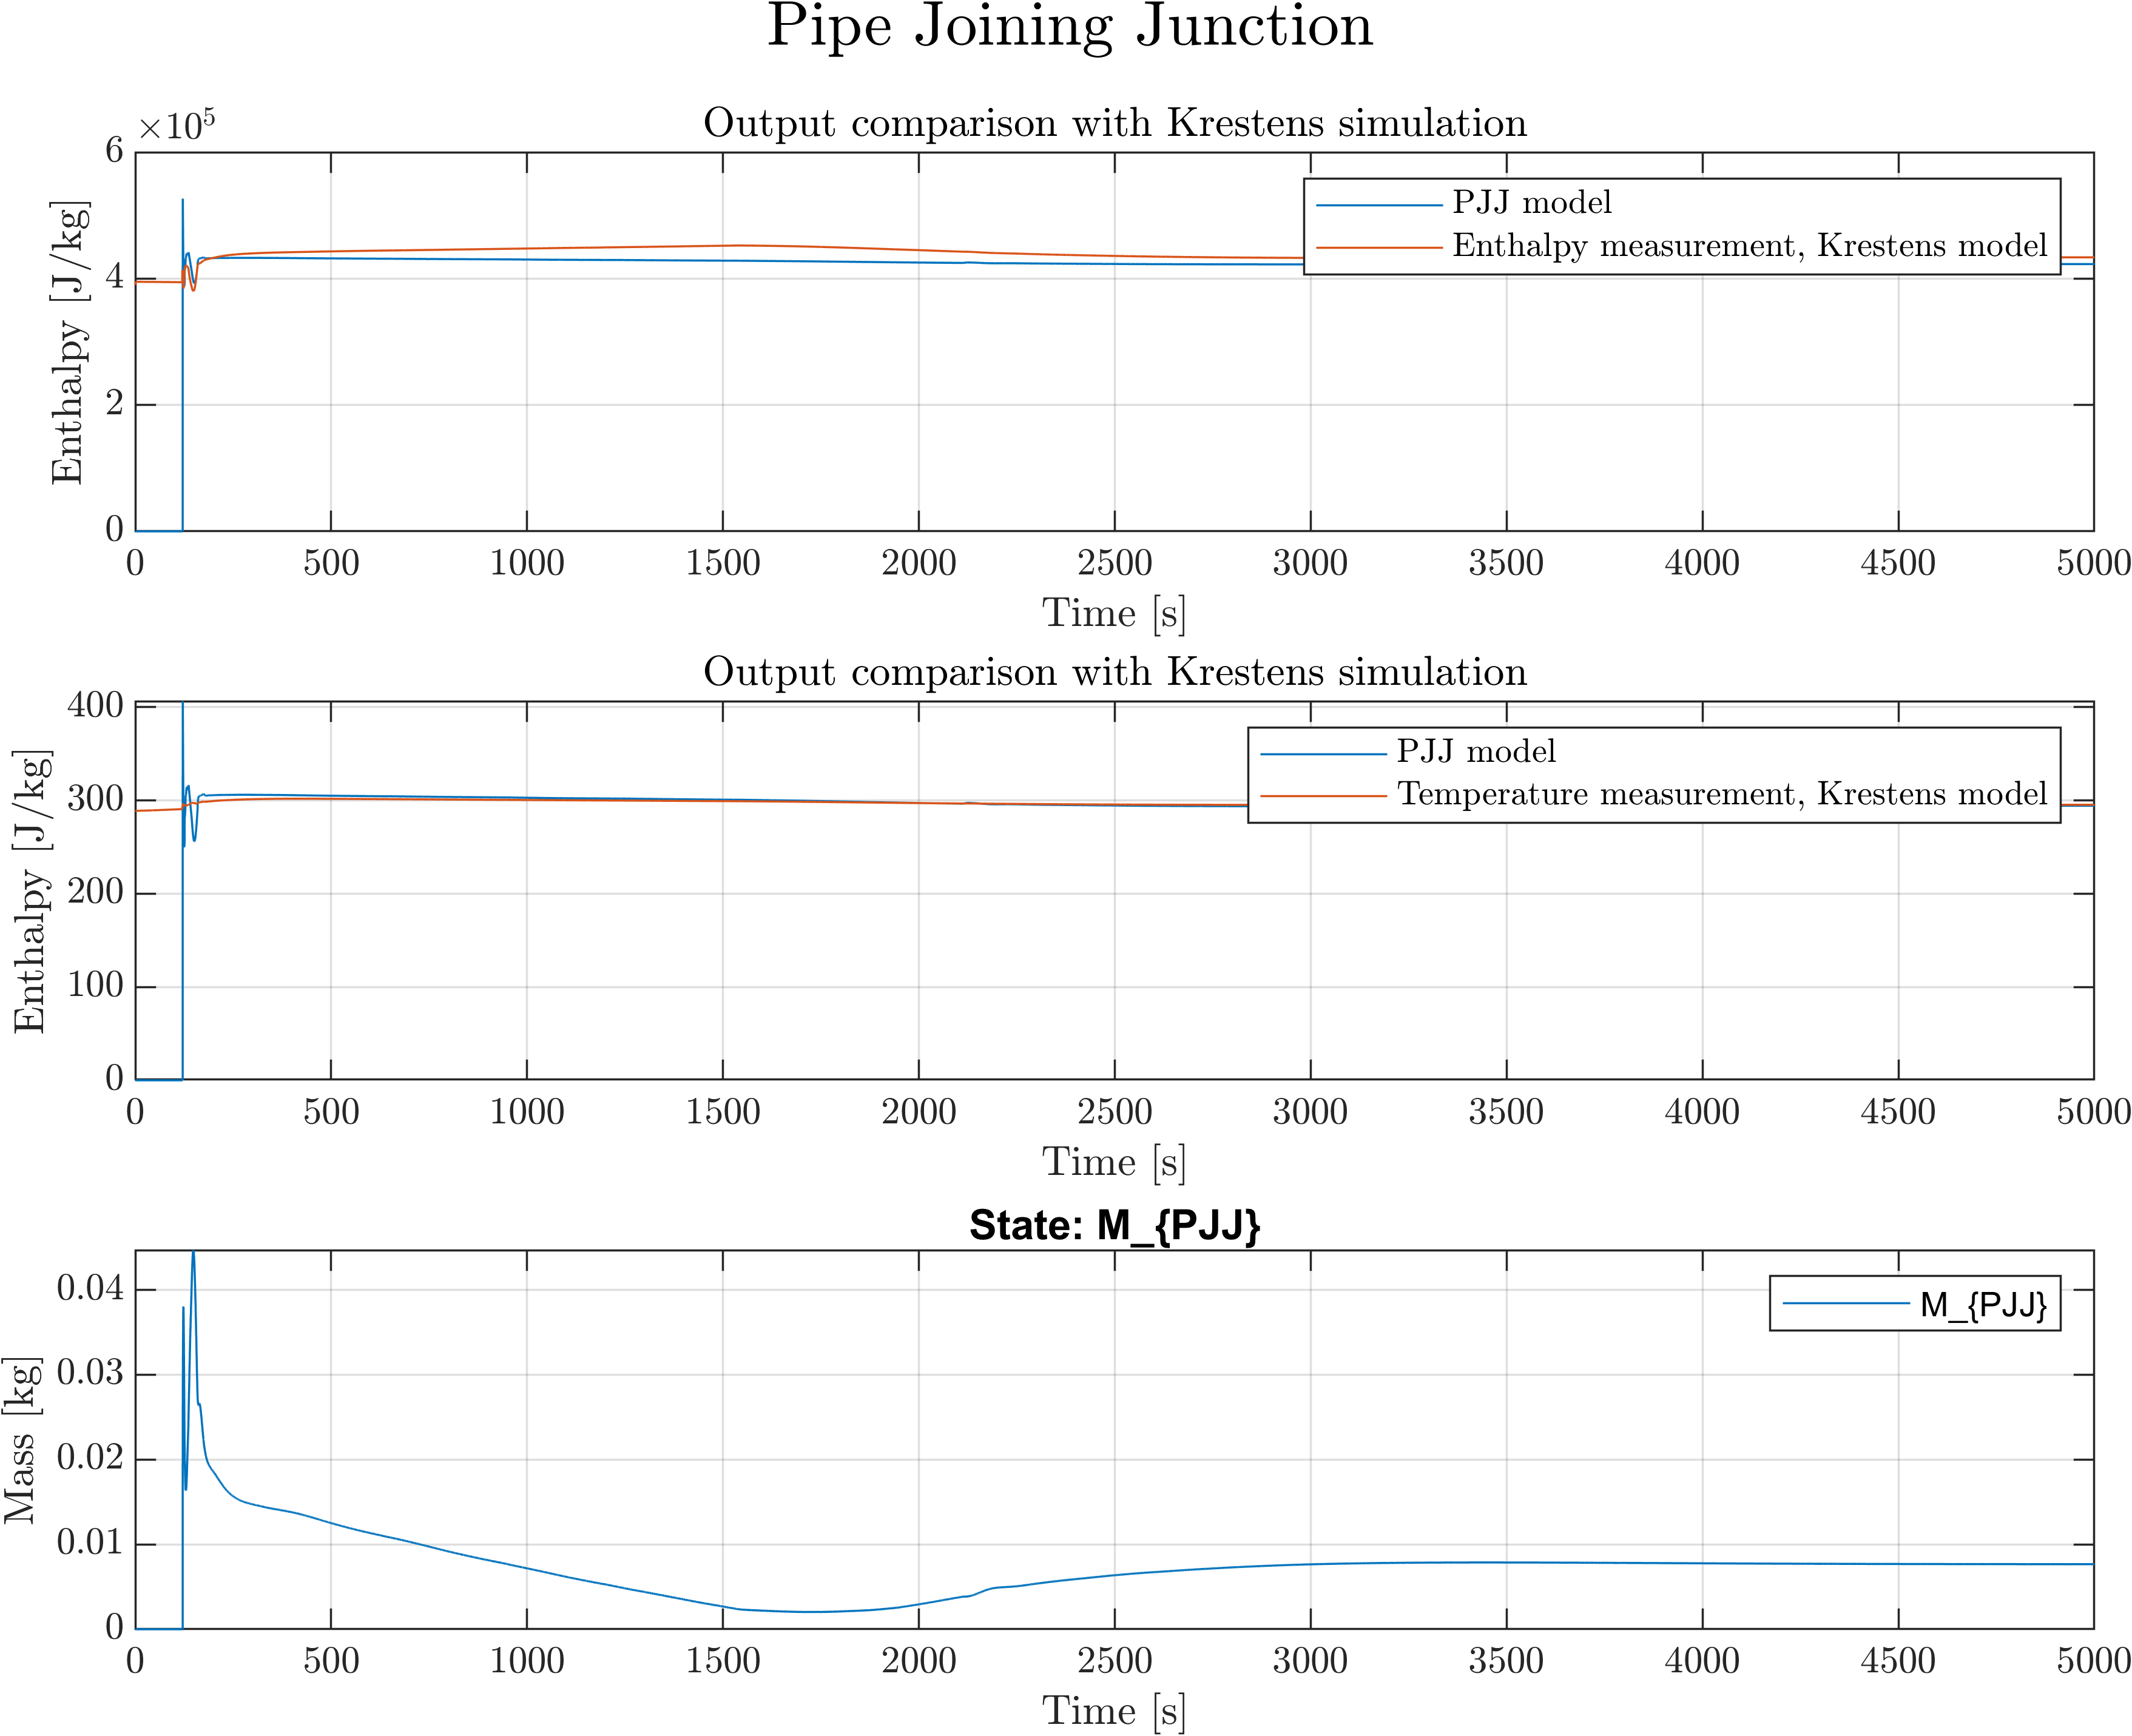
\includegraphics[width=1\textwidth]{Graphics/comp_test_pjj.png}
	\caption{Comparison of pjjModel outputs with HiFi component model of pipe joining junction}
	\label{fig:component_test_pjj}
\end{figure}
The pjjModel resembles the enthalpy and temperature outputs of the HiFi simulation in subplot 1 and 2 well from the time after 200 seconds. The transient is not great for the temperature comparison, however. This is likely due to initialisation of pjjModel is different from the Hifi model pipe joining junction.
In steady state the outputs are considered satisfactory.

\clearpage
\begin{figure}[h]
	\centering
	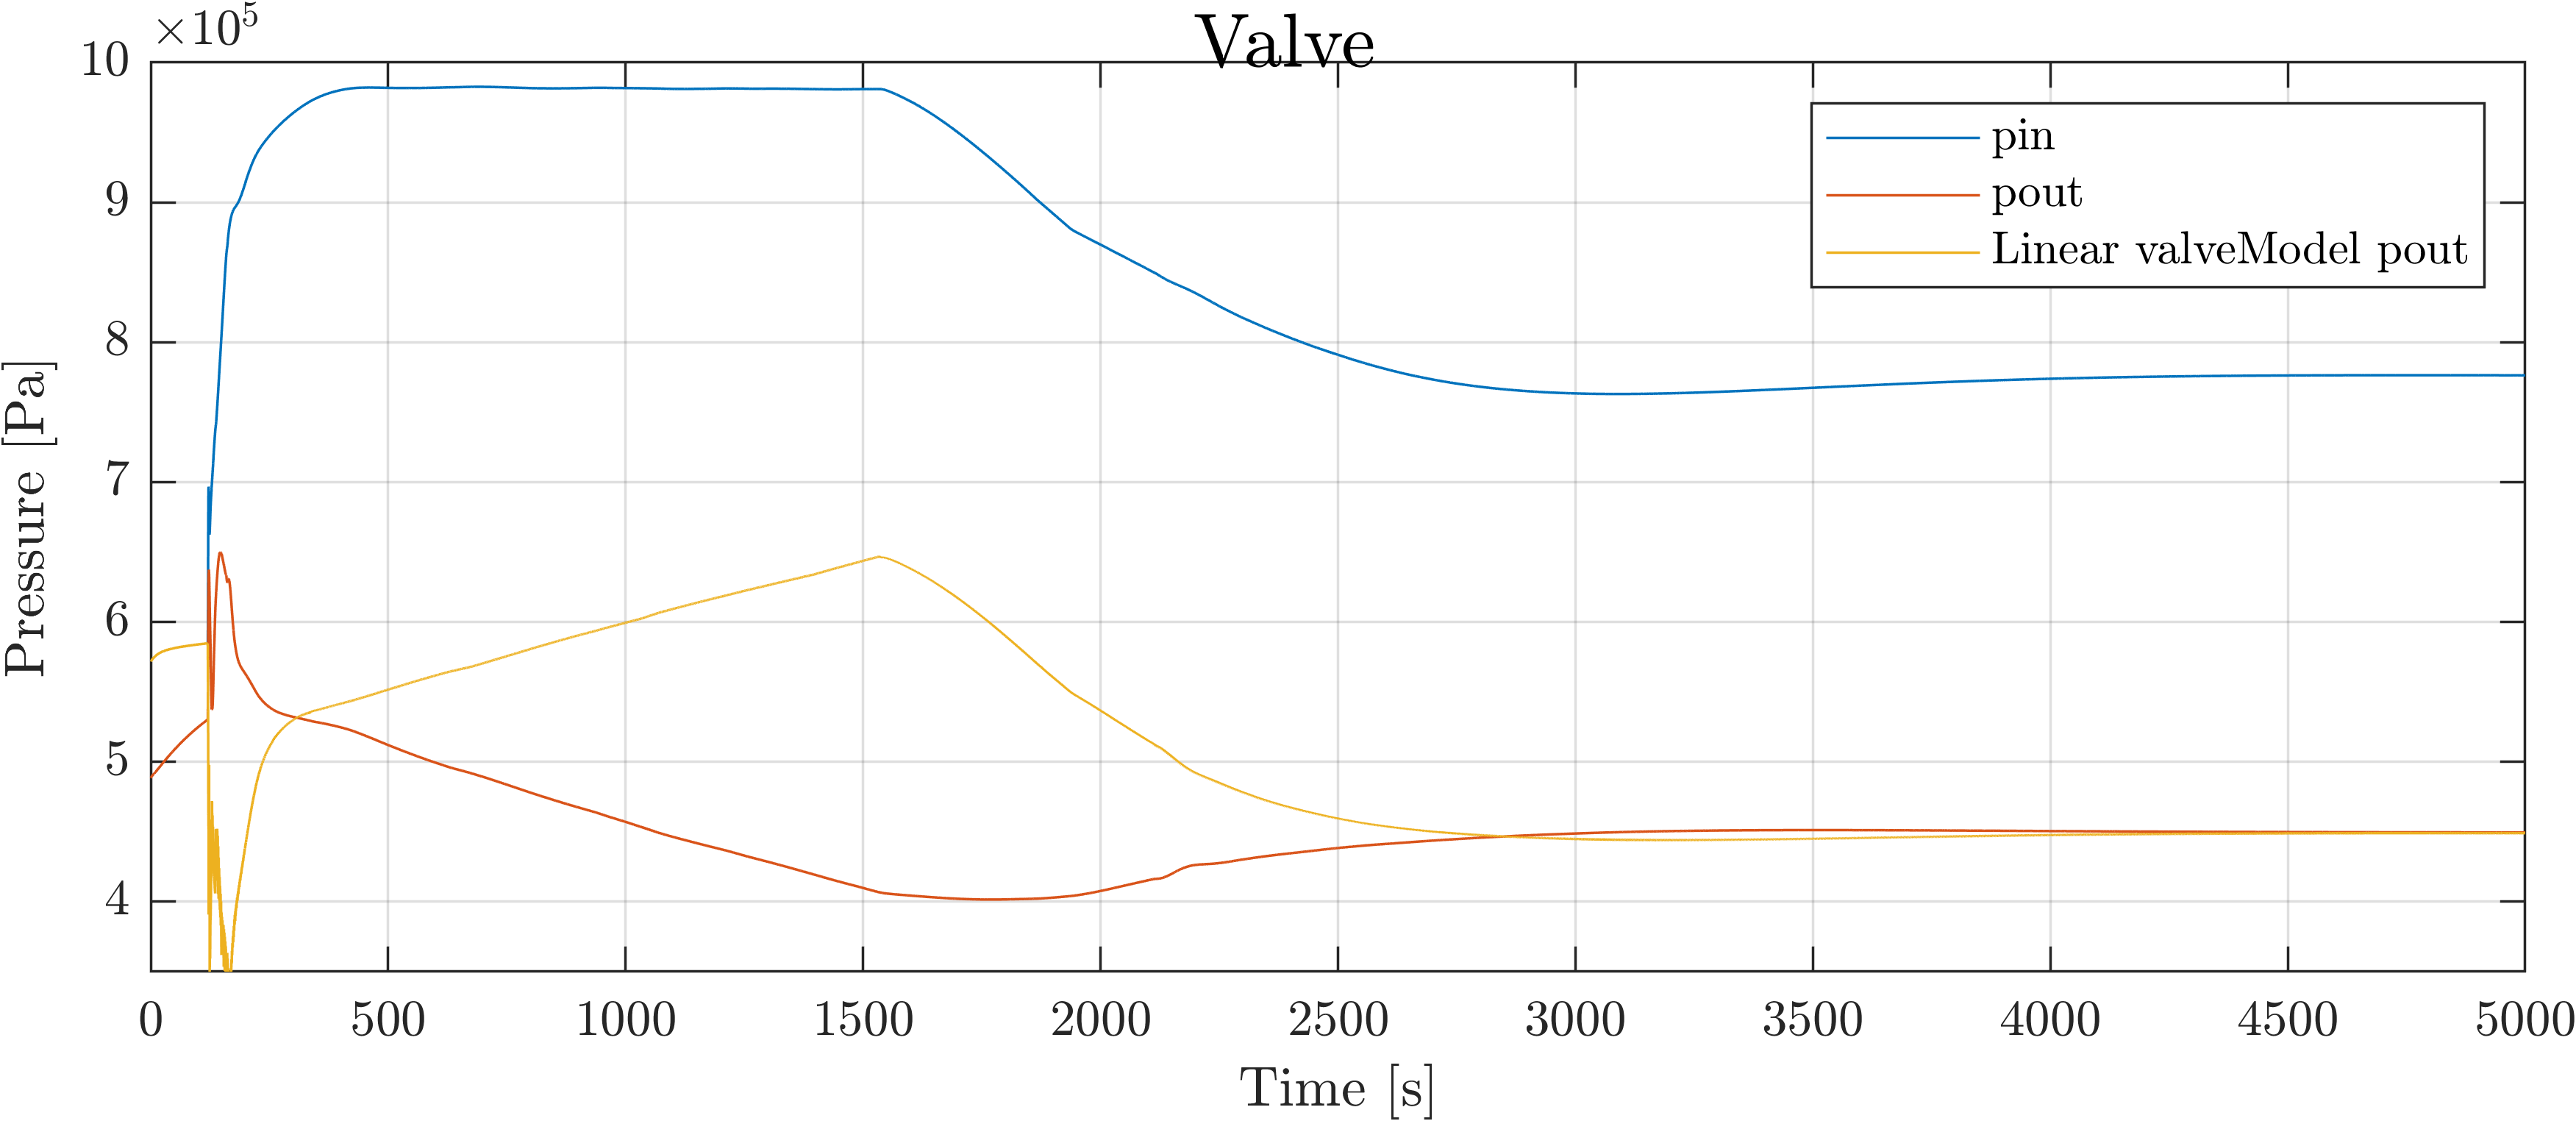
\includegraphics[width=1\textwidth]{Graphics/comp_test_val.png}
	\caption{Comparison of valveModel outputs with HiFi component model of valve}
	\label{fig:component_test_val}
\end{figure}
The valve model transient from 100 s to 2500 s is not great.
A probable cause of the so differing behavior in the transient phase, where the derives seem to have roughly the same absolut values but opposing signs could be that the equation for valveModel is only valid when there is flow through the valve. When the 'real' valve is closed the pressure drop across the valve can be any reasonable number, but there will not be a flow through it, and such \cref{eq:valve_pres3} for valveModel will not hold.

When debugging this transient, the equation that is base for the pressure out of the valveModel came in handy. It can be seen in \cref{eq:valve_pres3}.
\begin{equation}
	p_{out} = p_{in} - \dot{m}^2 \dfrac{v_{in}}{(\Theta \cdot K)^2} = p_{in} - \dot{m}^2 \cdot v_{in} \dfrac{1}{(\Theta \cdot K)^2} \label{eq:valve_pres3}
\end{equation}
The input pressure is plotted in \cref{fig:component_test_val}.
In the debugging it was observed was that the term $ \dfrac{1}{(\Theta \cdot K)^2} $ took up values above 1e10. This indicates that the valve model perhabs is not good enough for the model to be sufficiently accurate.
After fiddling with the constant K, the valve model ended up being accurate in steady state, as seen after 3000 s.

\clearpage
\begin{figure}[h]
	\centering
	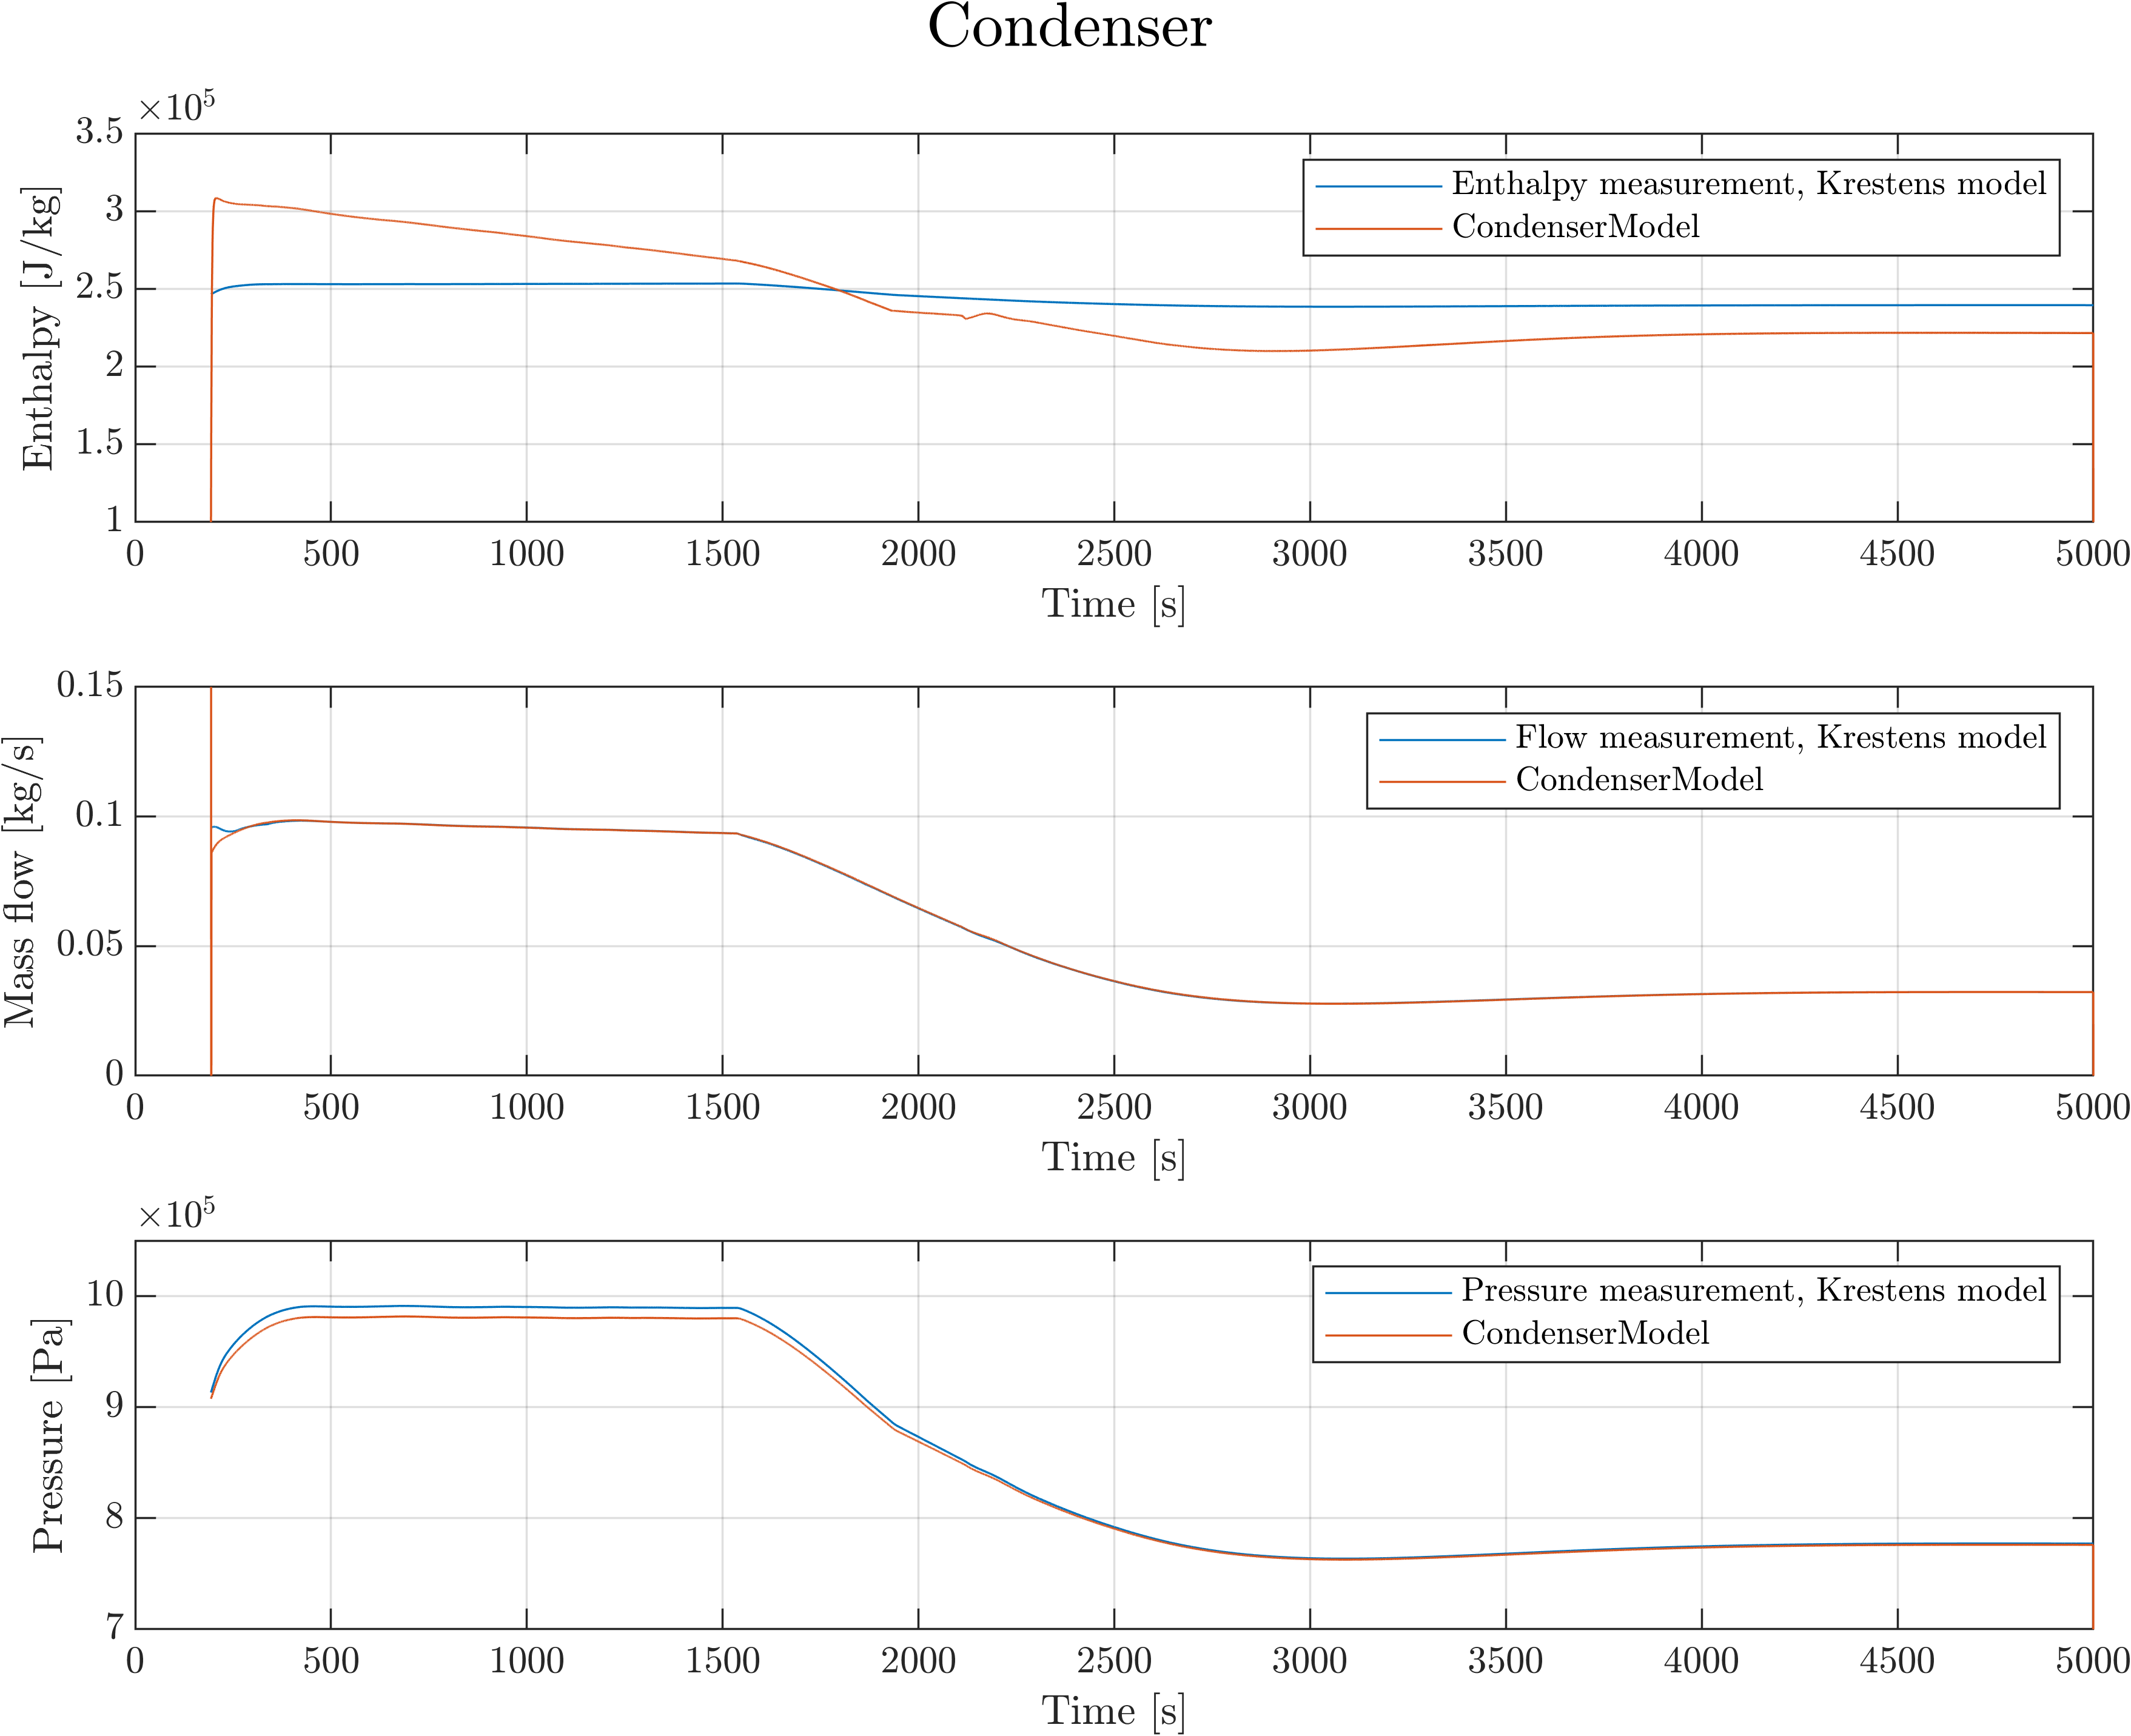
\includegraphics[width=1\textwidth]{Graphics/comp_test_ft.png}
	\caption{Comparison of flashtankModel outputs with HiFi component model of flash tank}
	\label{fig:component_test_ft}
\end{figure}
The flashtankModel accuracy is satisfactory as the enthalpies are very accurate. The mass flows deviate a bit in the transient phases - likely due to the lacking dynamics in the mass balance, but it is considered satisfactory anyway.


\clearpage
\begin{figure}[h]
	\centering
	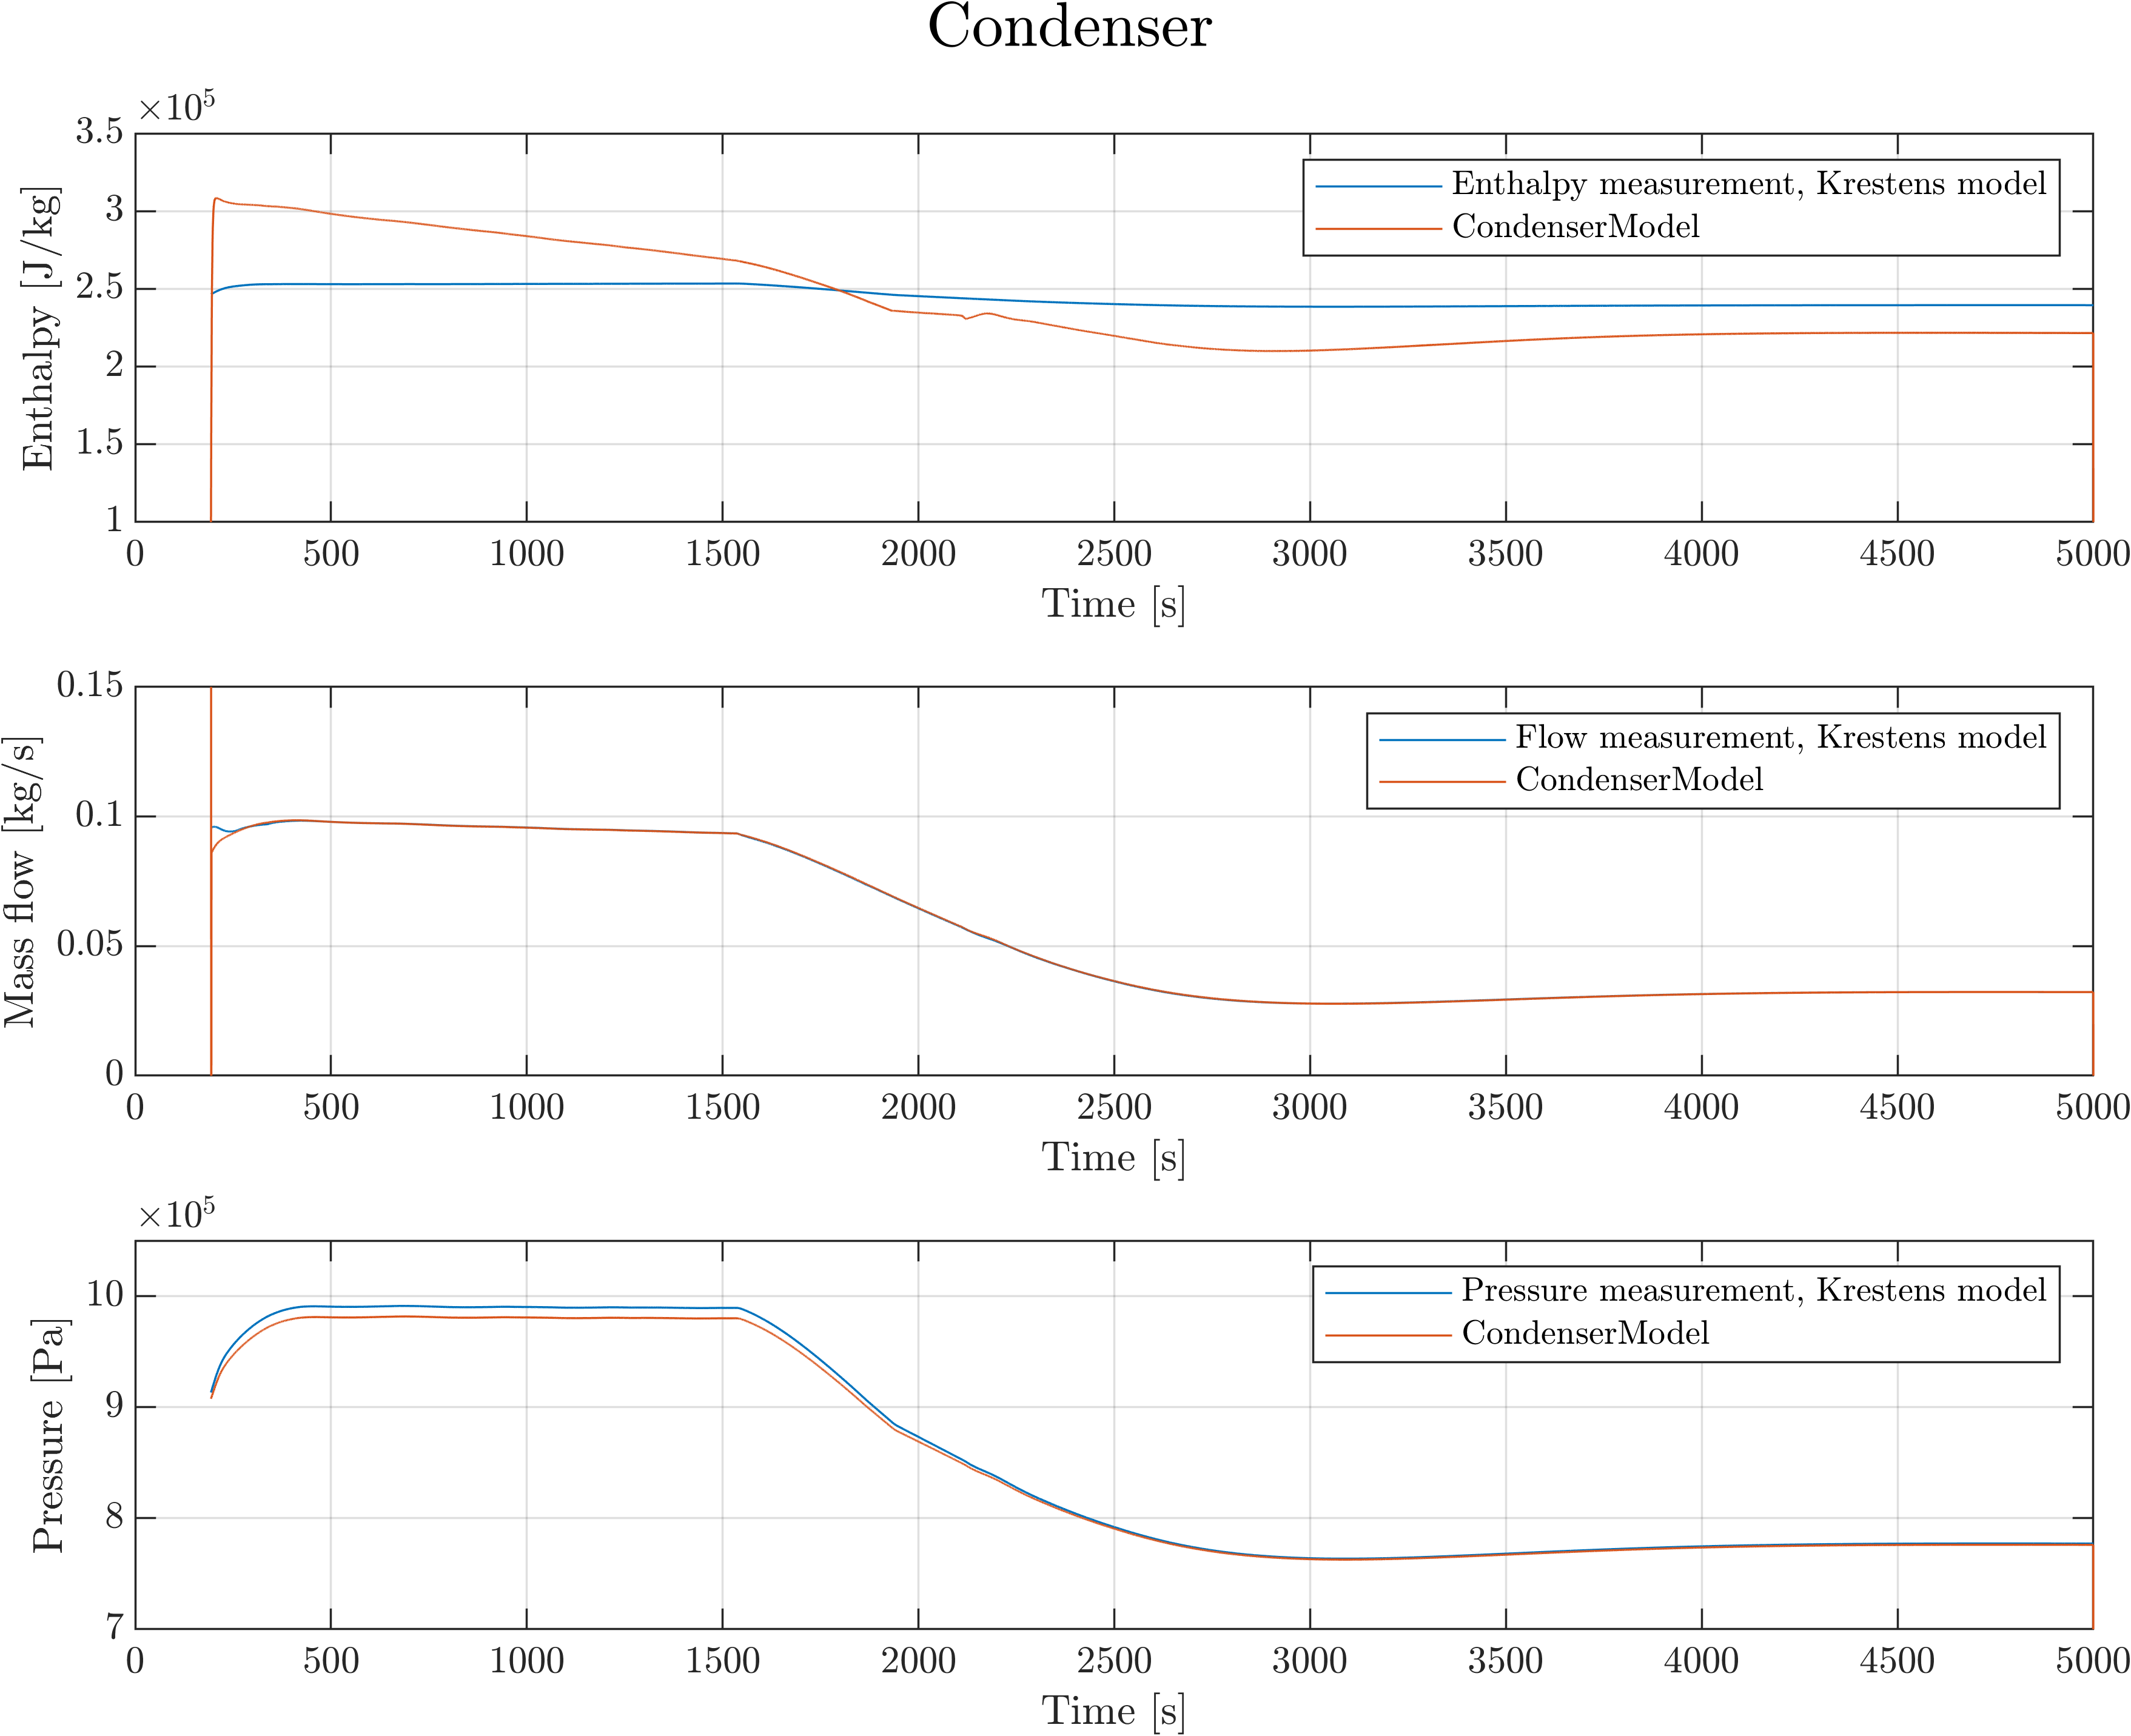
\includegraphics[width=1\textwidth]{Graphics/comp_test_con.png}
	\caption{Comparison of condenserModel outputs with HiFi component model of condenser}
	\label{fig:component_test_con}
\end{figure}

The condenser model accuracy is good for the mass flow and pressure as seen in \cref{fig:component_test_con} in subplot 2 and 3. The enthalpy accuracy is less accurate, both in the transient phase around 100-1750 s and in steady state. However it is considered suffient as the steady state value about 10\% off.
The accuracy in the steady state enthalpy was not based on the heat transfer coefficients from \cref{sec:condenser}. With those there were significant offset errors. They were varied by trial and error to obtain more accurate steady state behavior - especially with regards to the enthalpy output.


\clearpage
\begin{figure}[h]
	\centering
	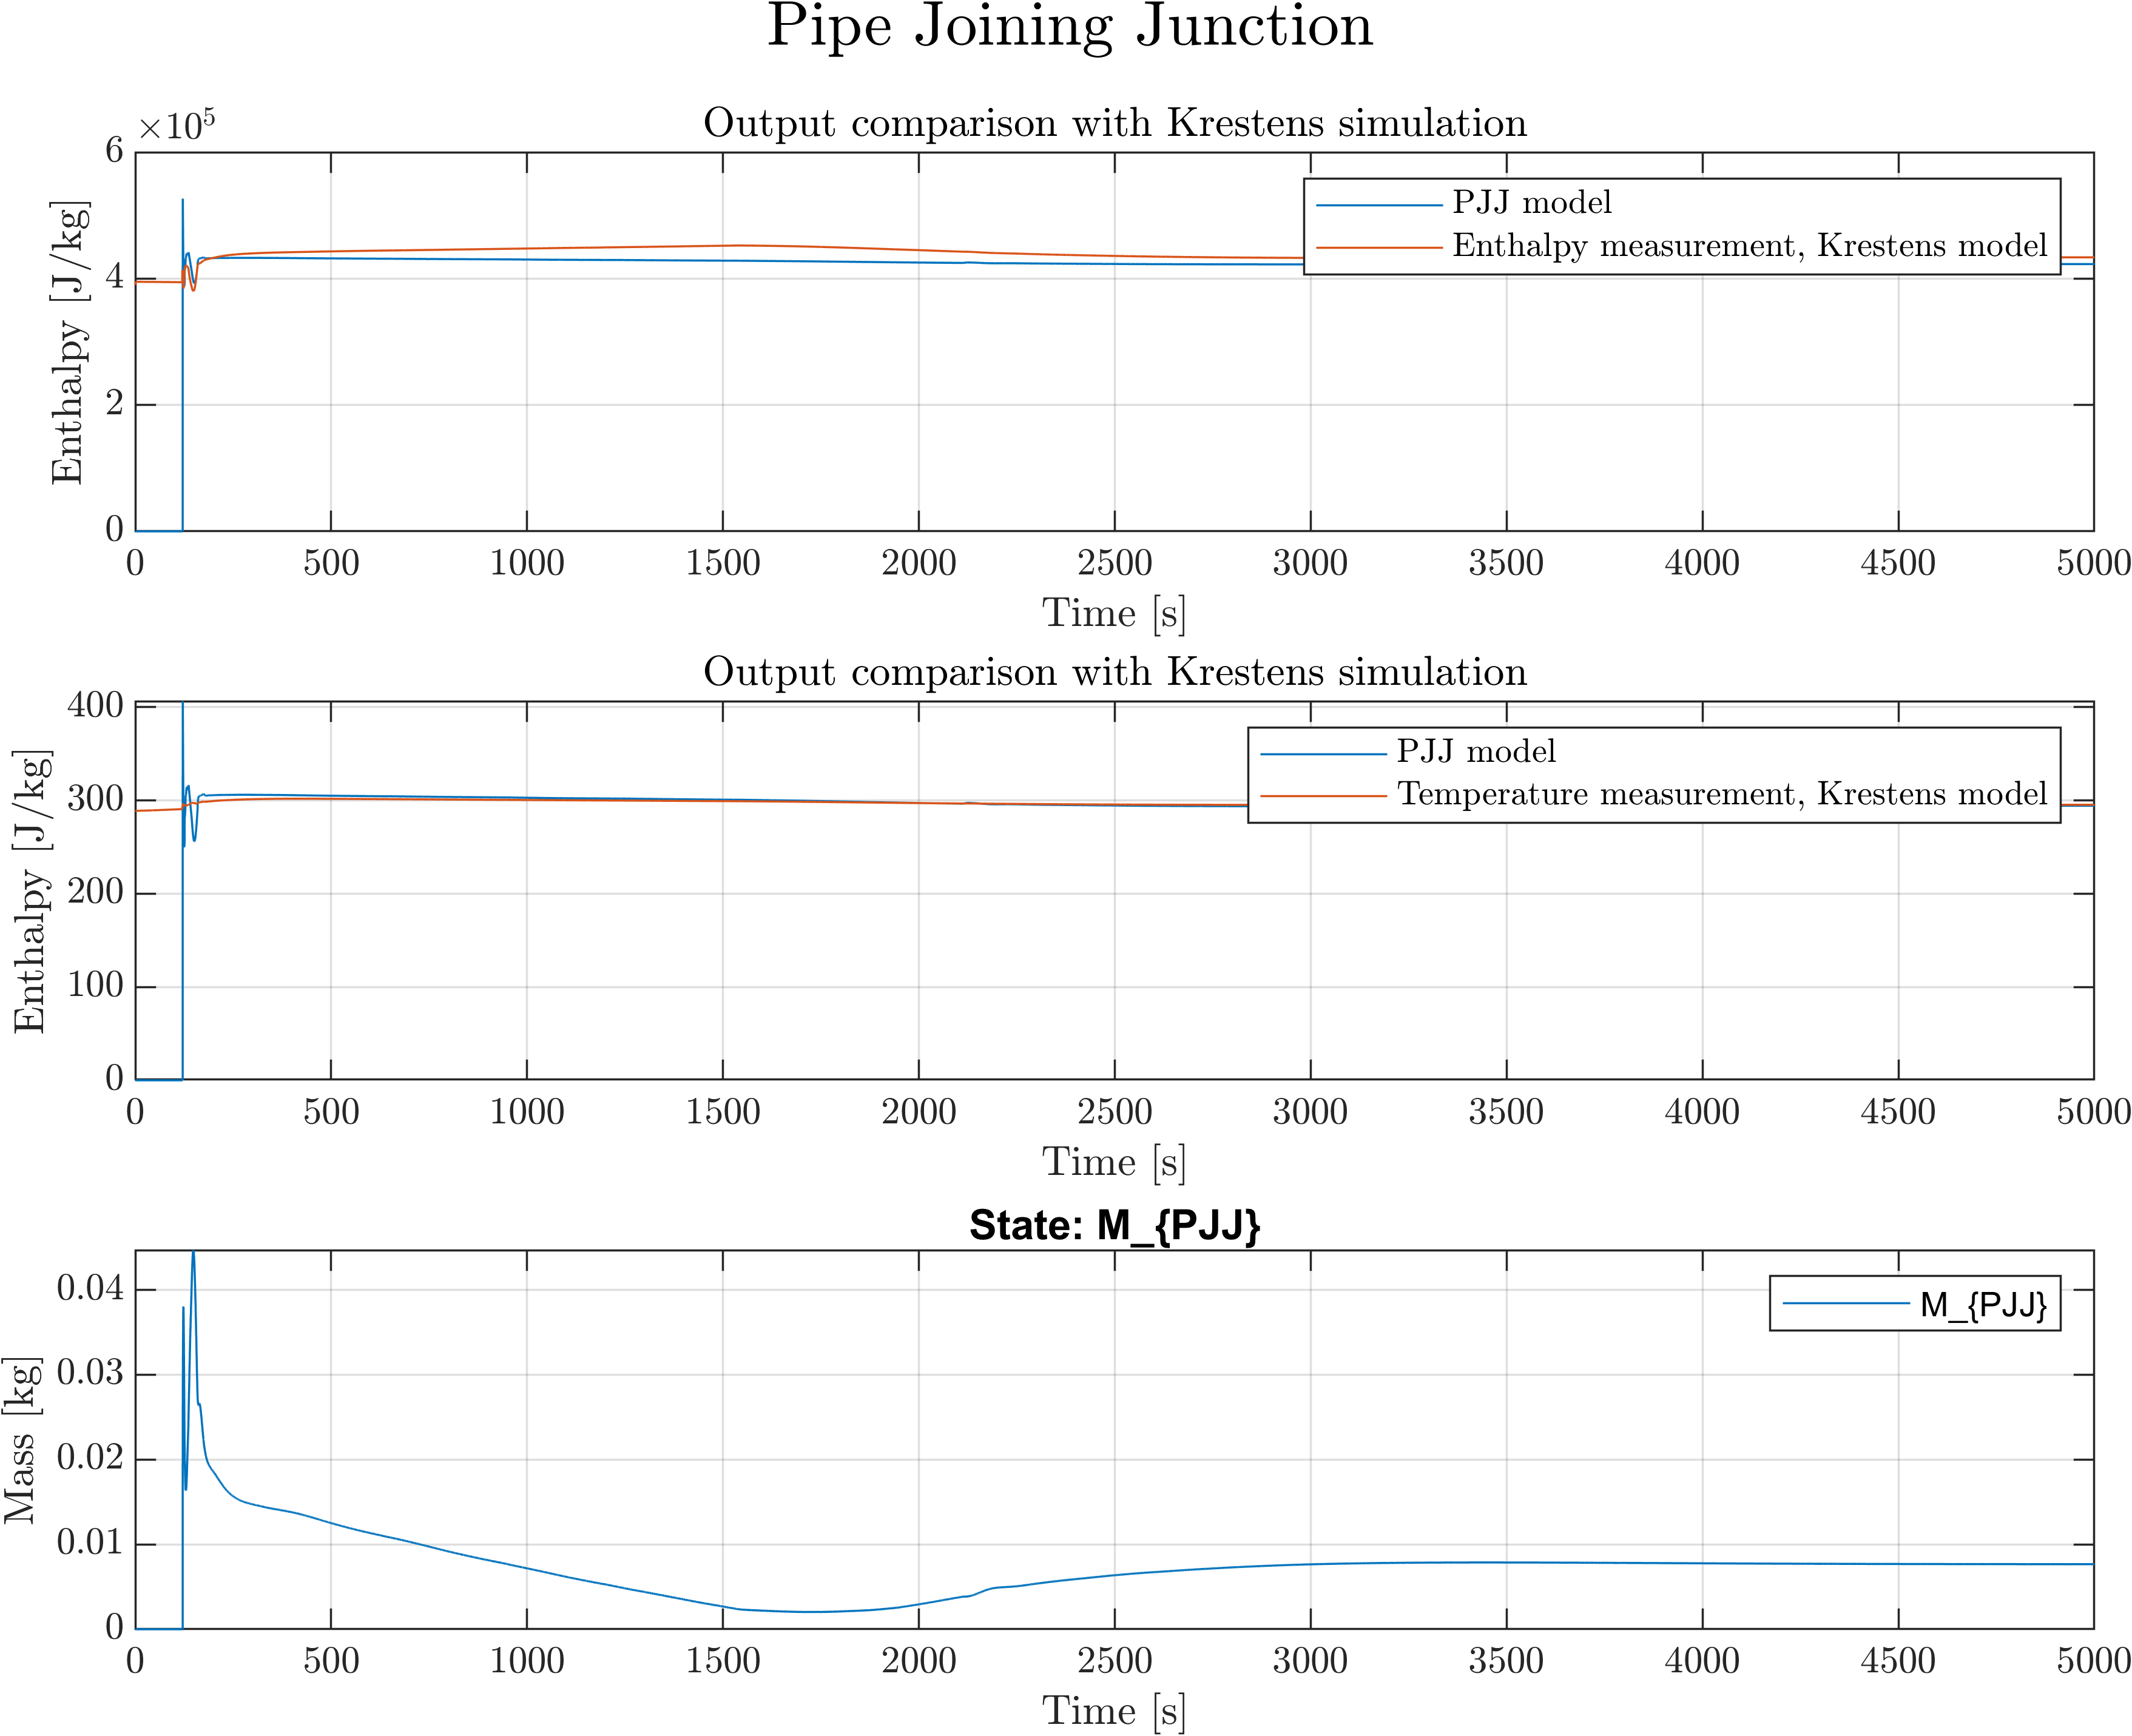
\includegraphics[width=1\textwidth]{Graphics/comp_test_box.png}
	\caption{Comparison of boxModel outputs with HiFi component model of box}
	\label{fig:component_test_box}
\end{figure}

The boxModel behavior is good in the sense that is seems like there is only more or less a constant offset between the boxModel outputs and the Hifi Model. A bit of fiddling with some of the constants in the boxModel might mitigate the offset error even more.

\clearpage
\begin{figure}[h]
	\centering
	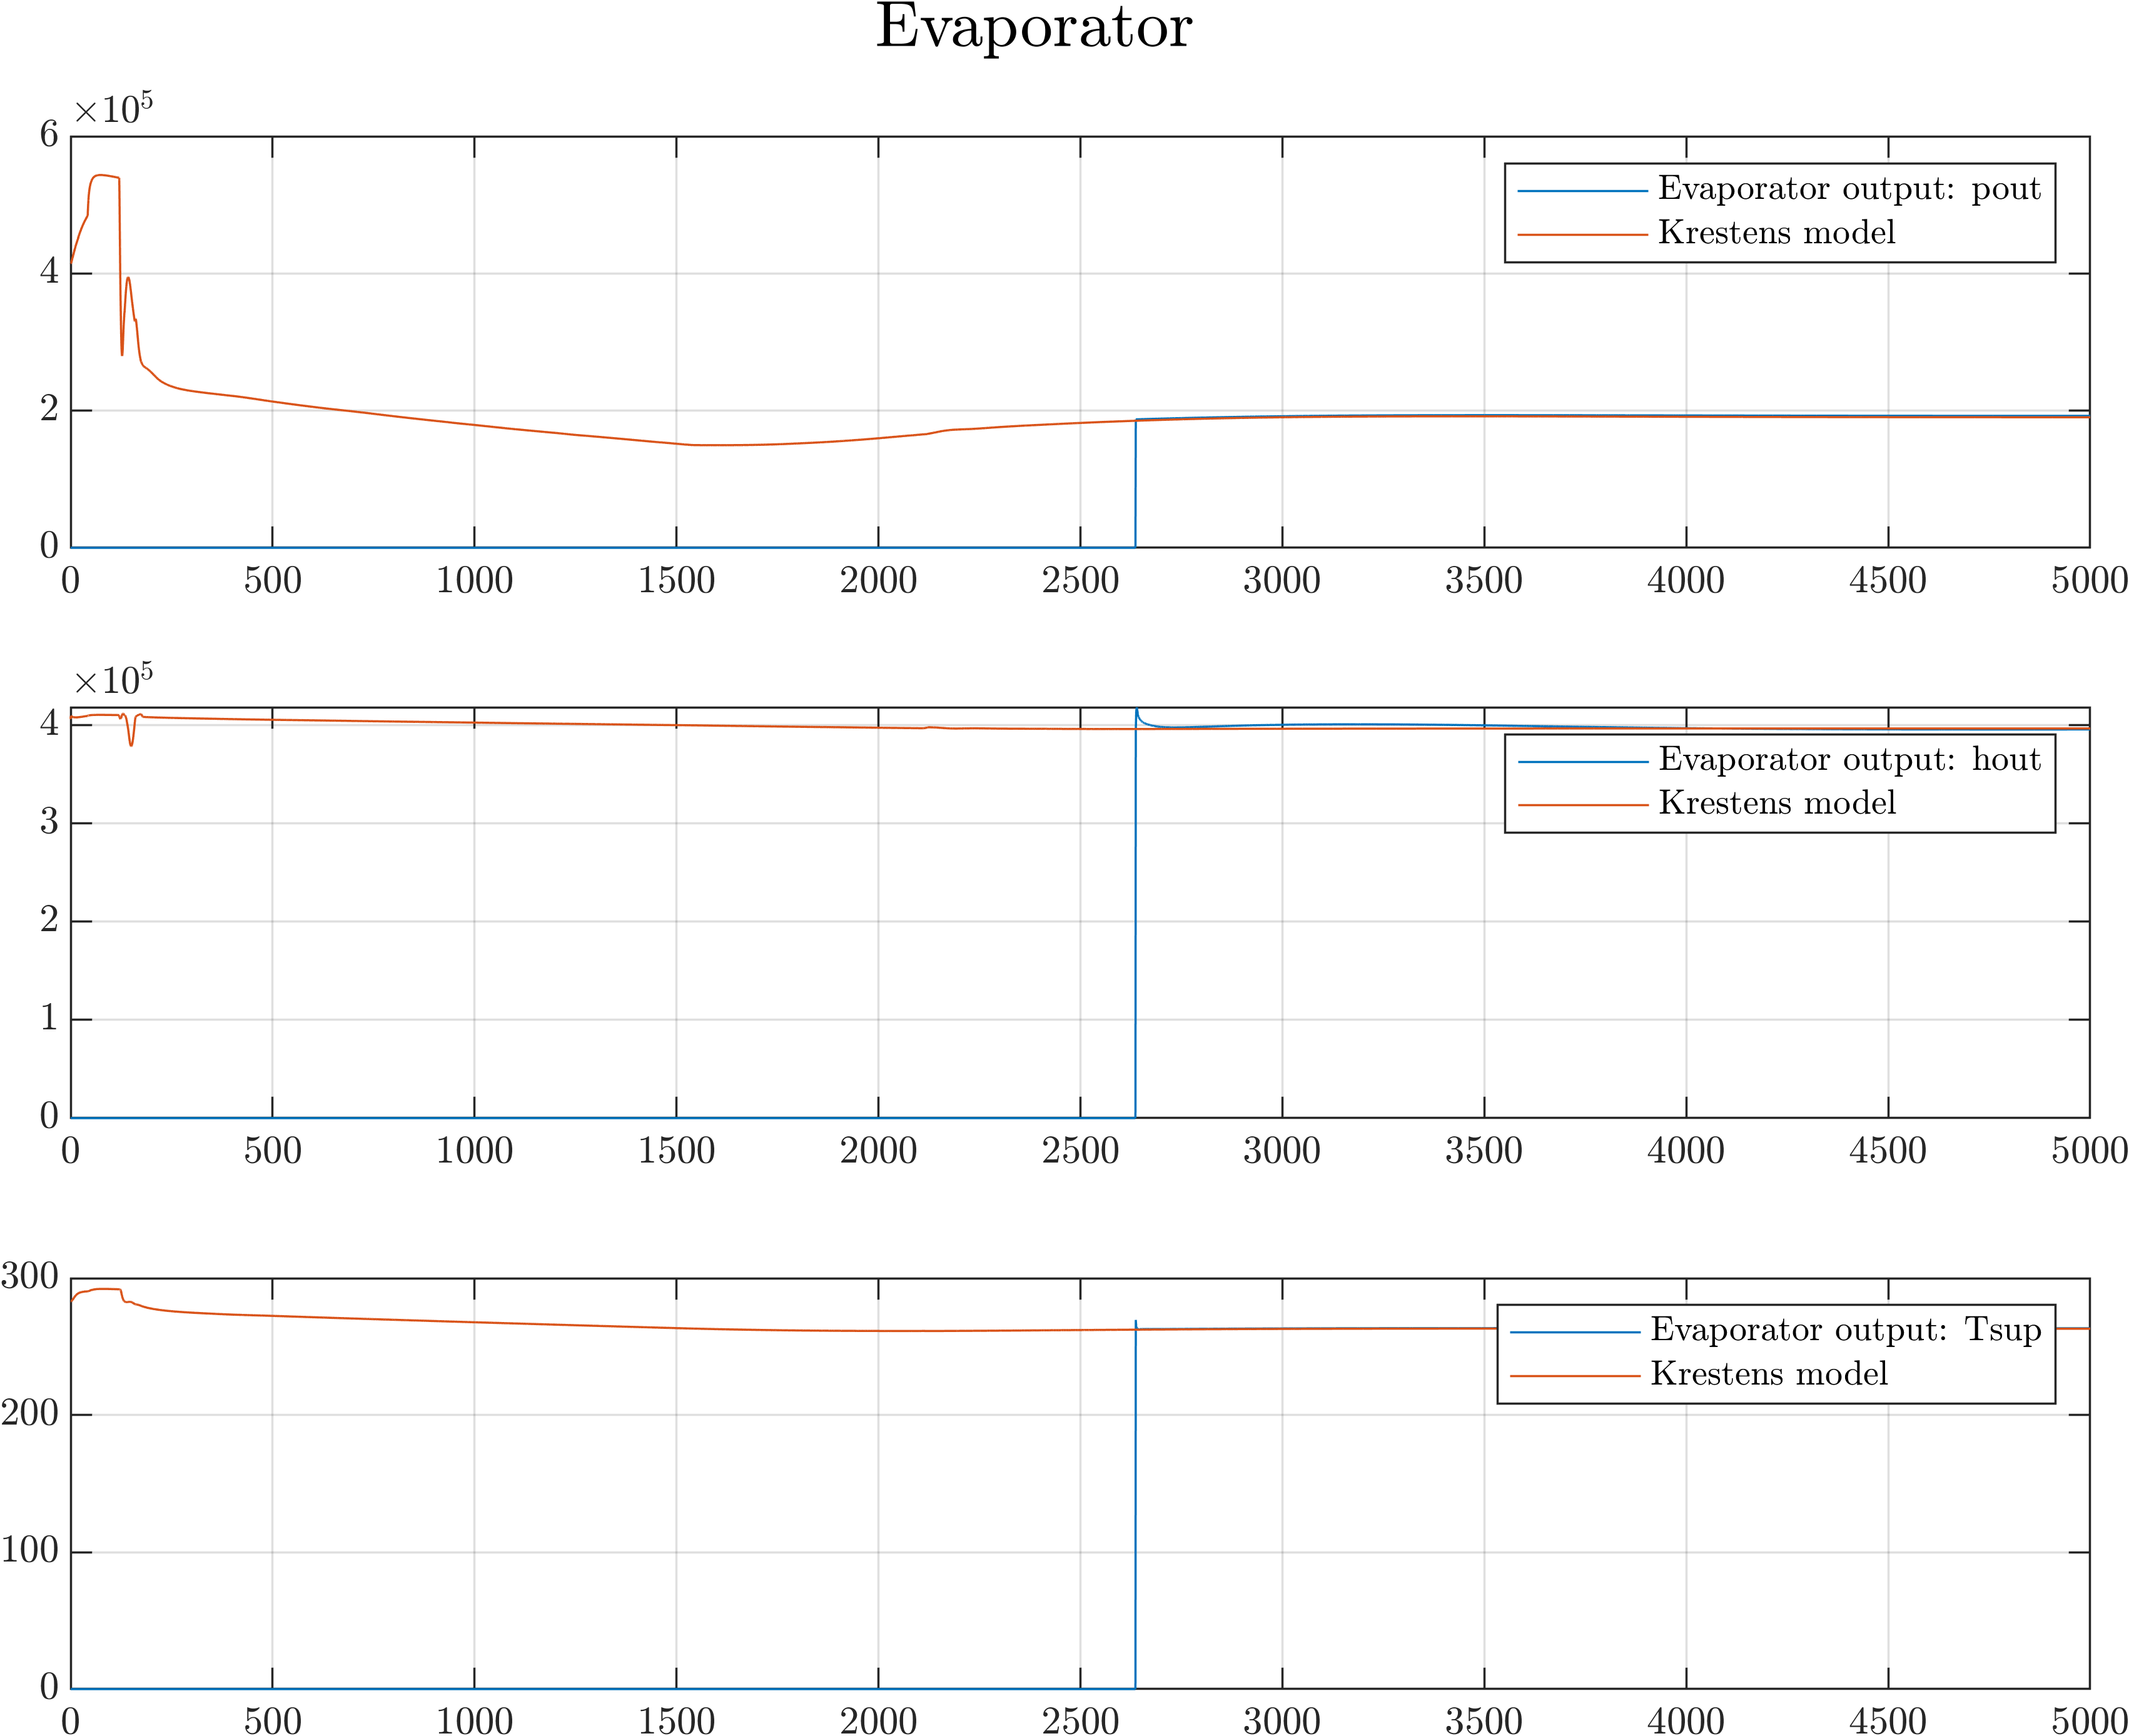
\includegraphics[width=1\textwidth]{Graphics/comp_test_eva.png}
	\caption{Comparison of evaporatorModel outputs with HiFi component model of evaporator}
	\label{fig:component_test_eva}
\end{figure}
The evaporator model could not run in the early phases of the input sequences as some of the look-up tables got out of their range. Thus the model is only evaluated from time 2600 s.
In the evaluated time the model shows satisfactory accuracy for both pressure, enthalpy and supply temperature


%comp_test_box.png
%comp_test_com.png
%comp_test_con.png
%comp_test_eva.png
%comp_test_ft.png
%comp_test_pjj.png
%comp_test_val.png

%First comes two plots with the output pressure being as in line 158 in \cref{fig:evapotest1_code}, \cref{fig:evapotest_plot1} showing the simulation with a start around time t= 2637 s and to the end.
%
%\begin{figure}[h]
%	\centering
%	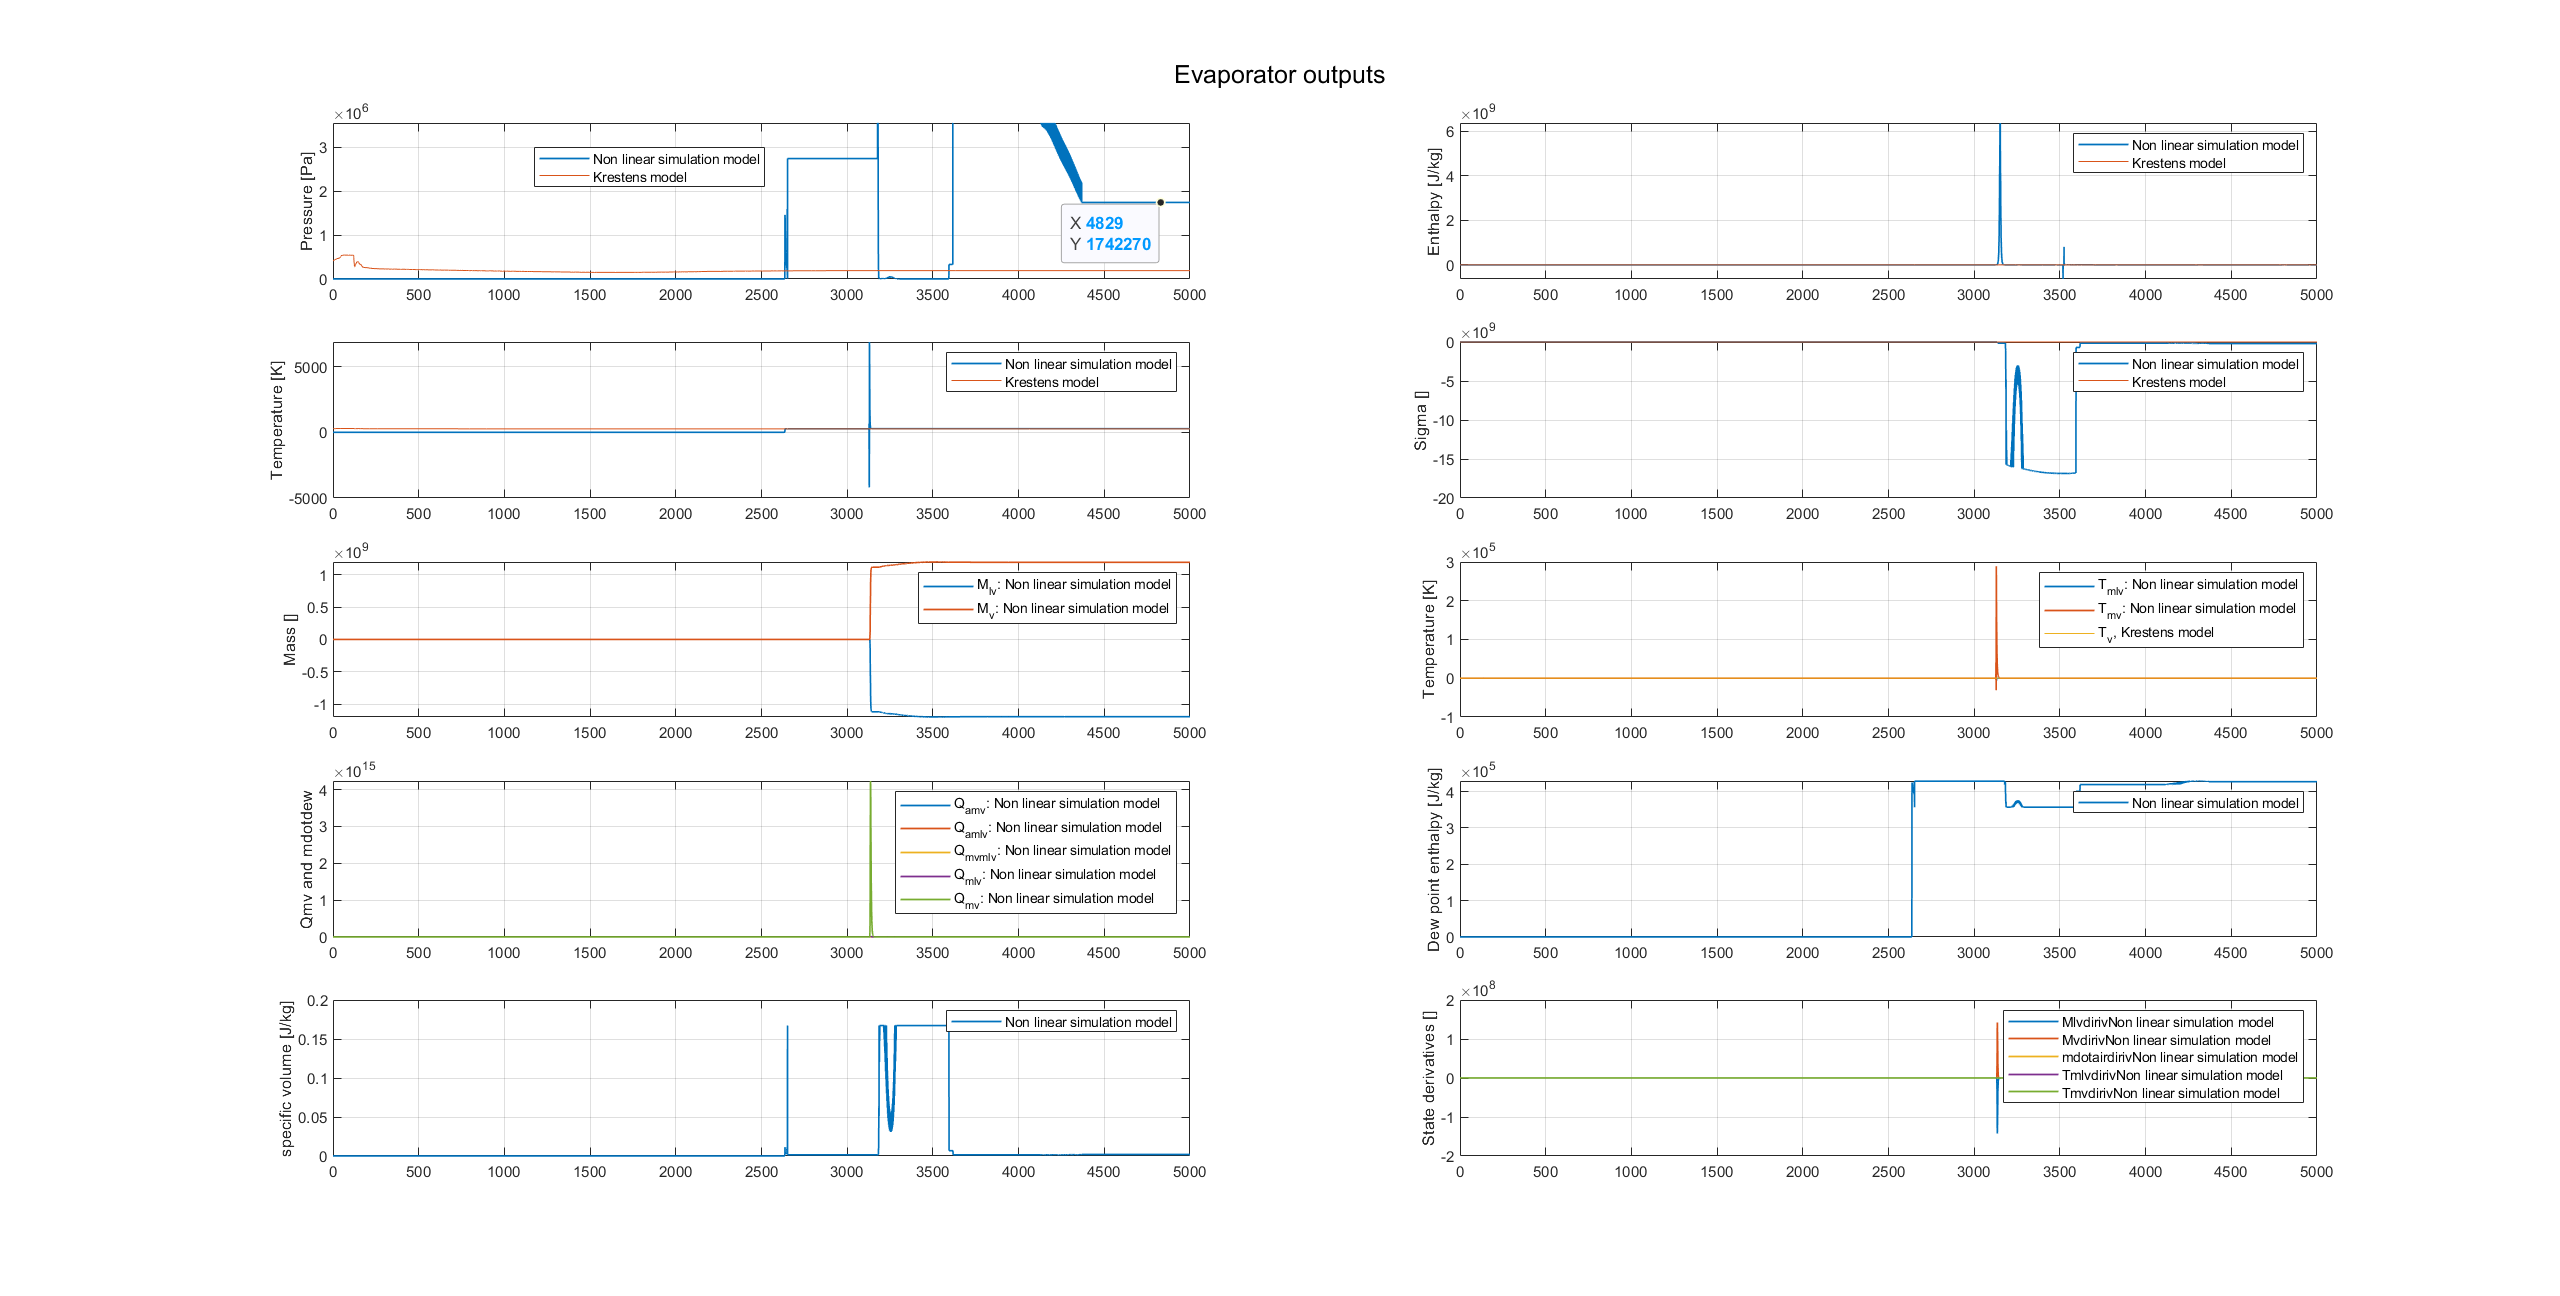
\includegraphics[width=2.1\textwidth]{Tests/Evapo_test1/plot_unstable.png}
%	\caption{Outputs with pressure out being a table lookup}
%	\label{fig:evapotest_plot1}
%\end{figure}
%
%Here if the upper left plot is observed, the output pressure of the evaporator model shows unstable behavior and eventual settling around a way to high value of 17.4 bar = 1740000 Pa.
%
%\begin{figure}[h]
%	\centering
%	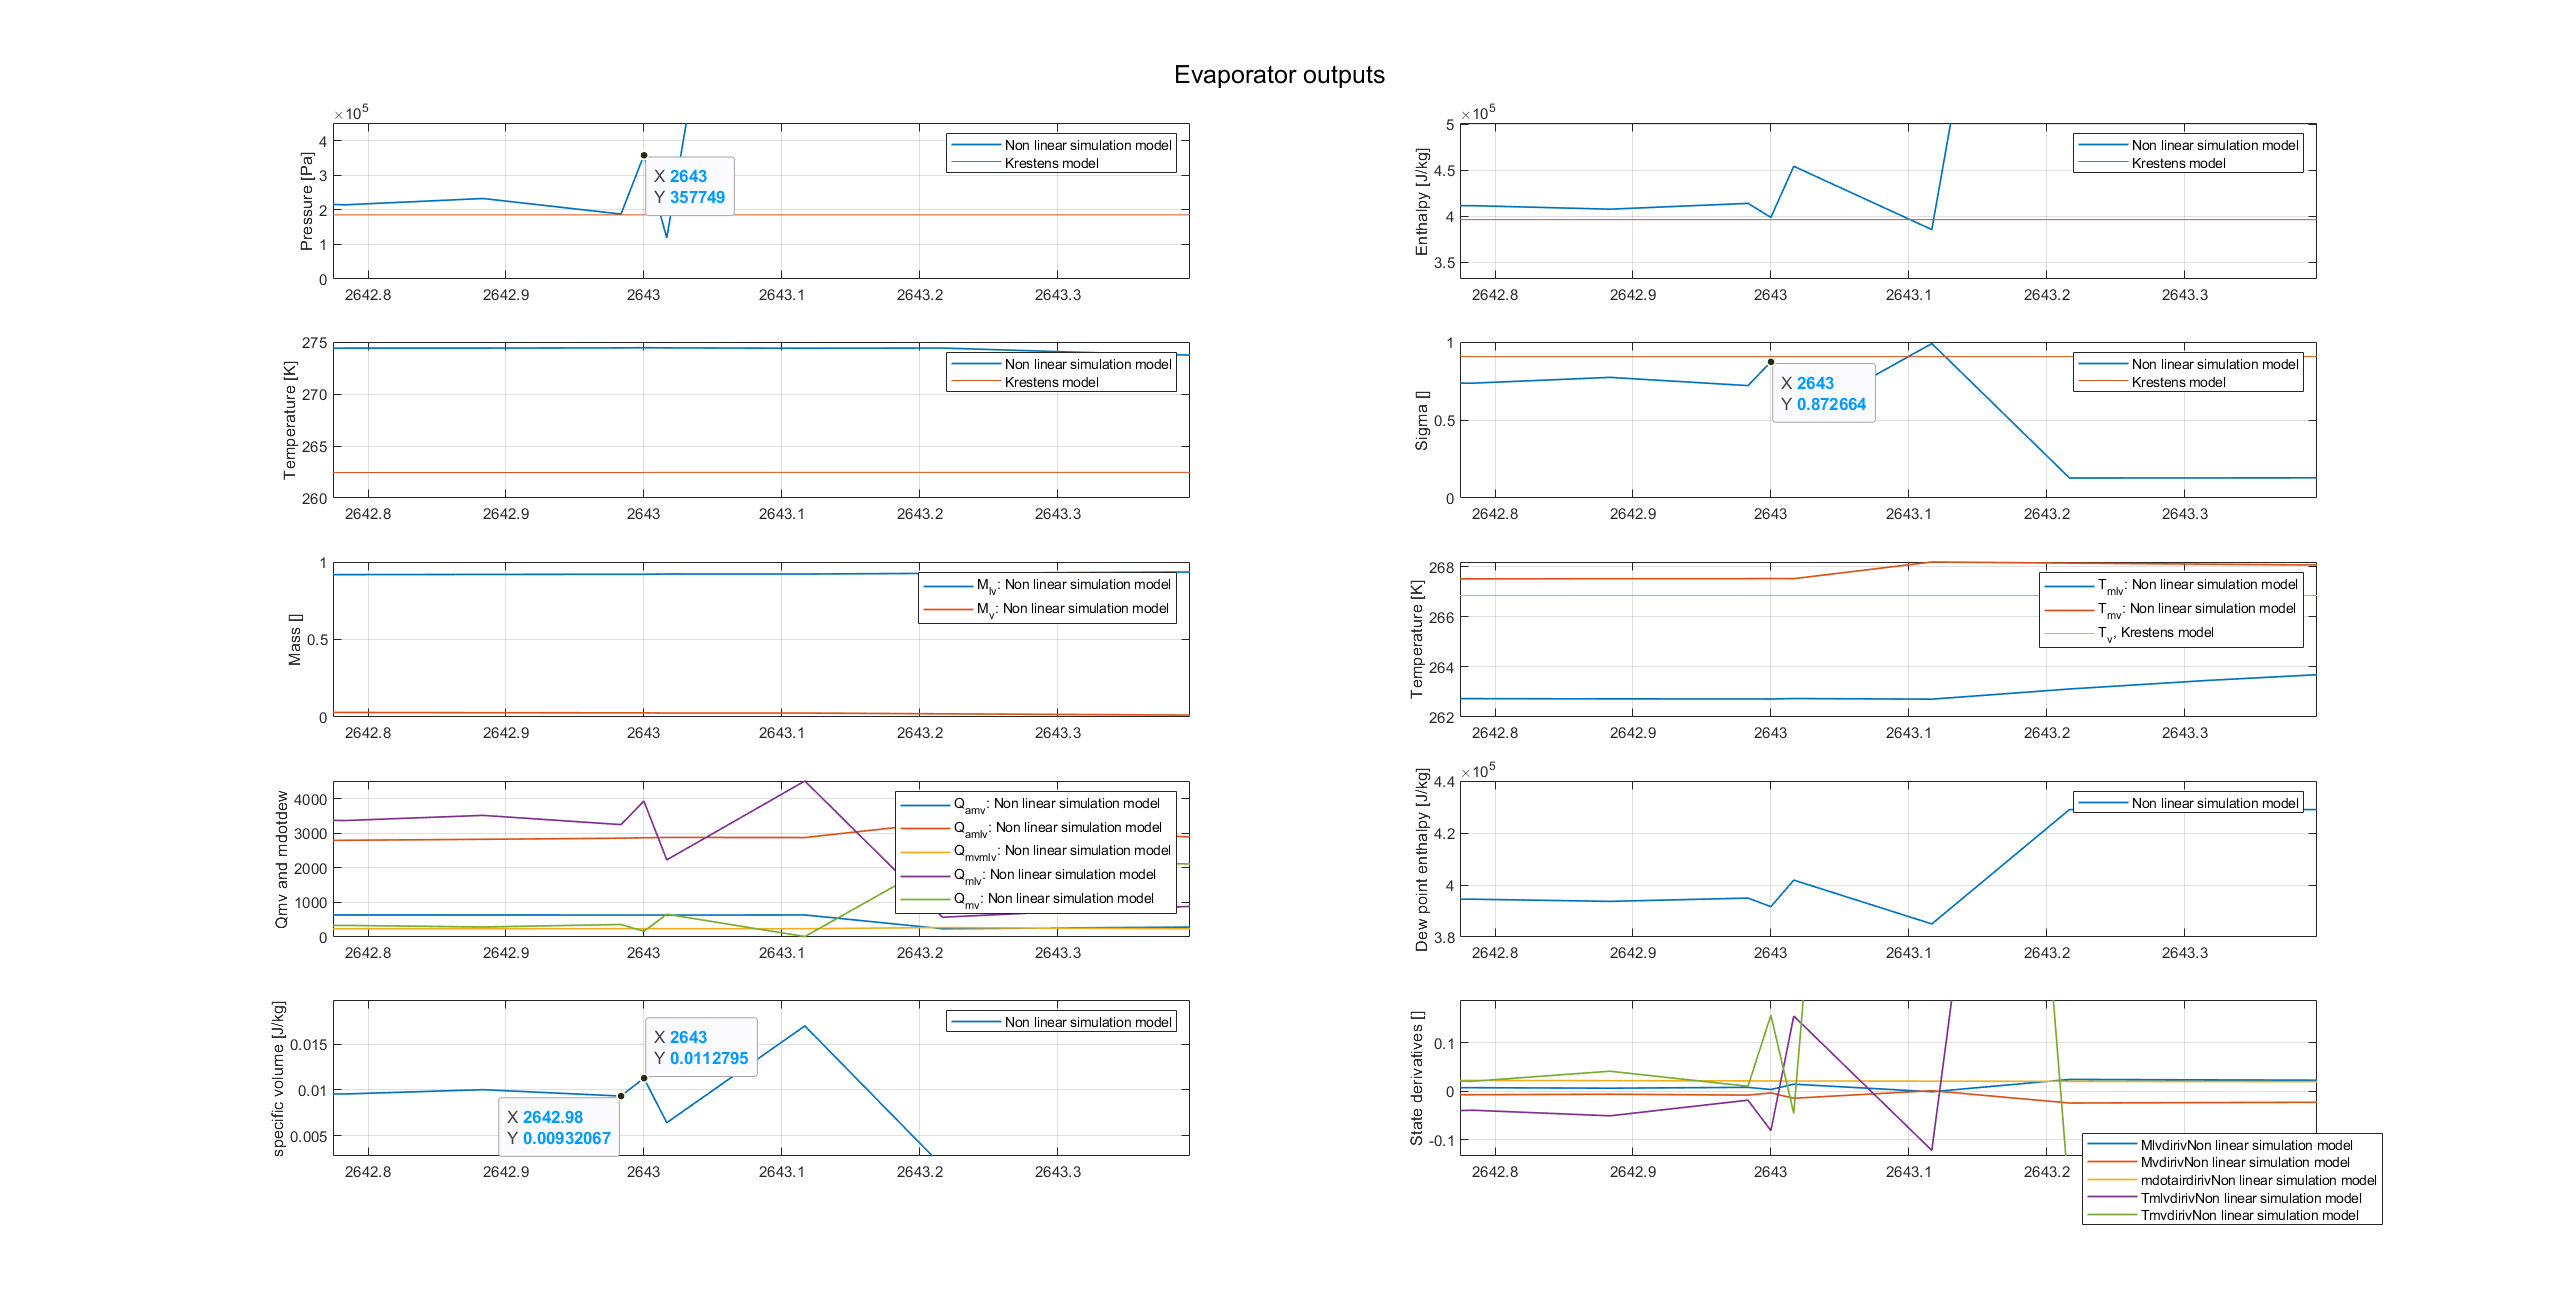
\includegraphics[width=2.1\textwidth]{Tests/Evapo_test1/plot_unstable_zoomed.png}
%	\caption{Zoomed version of \cref{fig:evapotest_plot1}}
%	\label{fig:evapotest_plot2}
%\end{figure}
%In \cref{fig:evapotest_plot2} is a zoom around time t = 2643 s where the simulation proves to start be unstable. From debugging, a sense of a positive feedback loop between look up table from the specific volume and the pressure was assumed. This was the root of the idea of setting $ p_{out} = p_{in} $
%
%\begin{figure}[h]
%	\centering
%	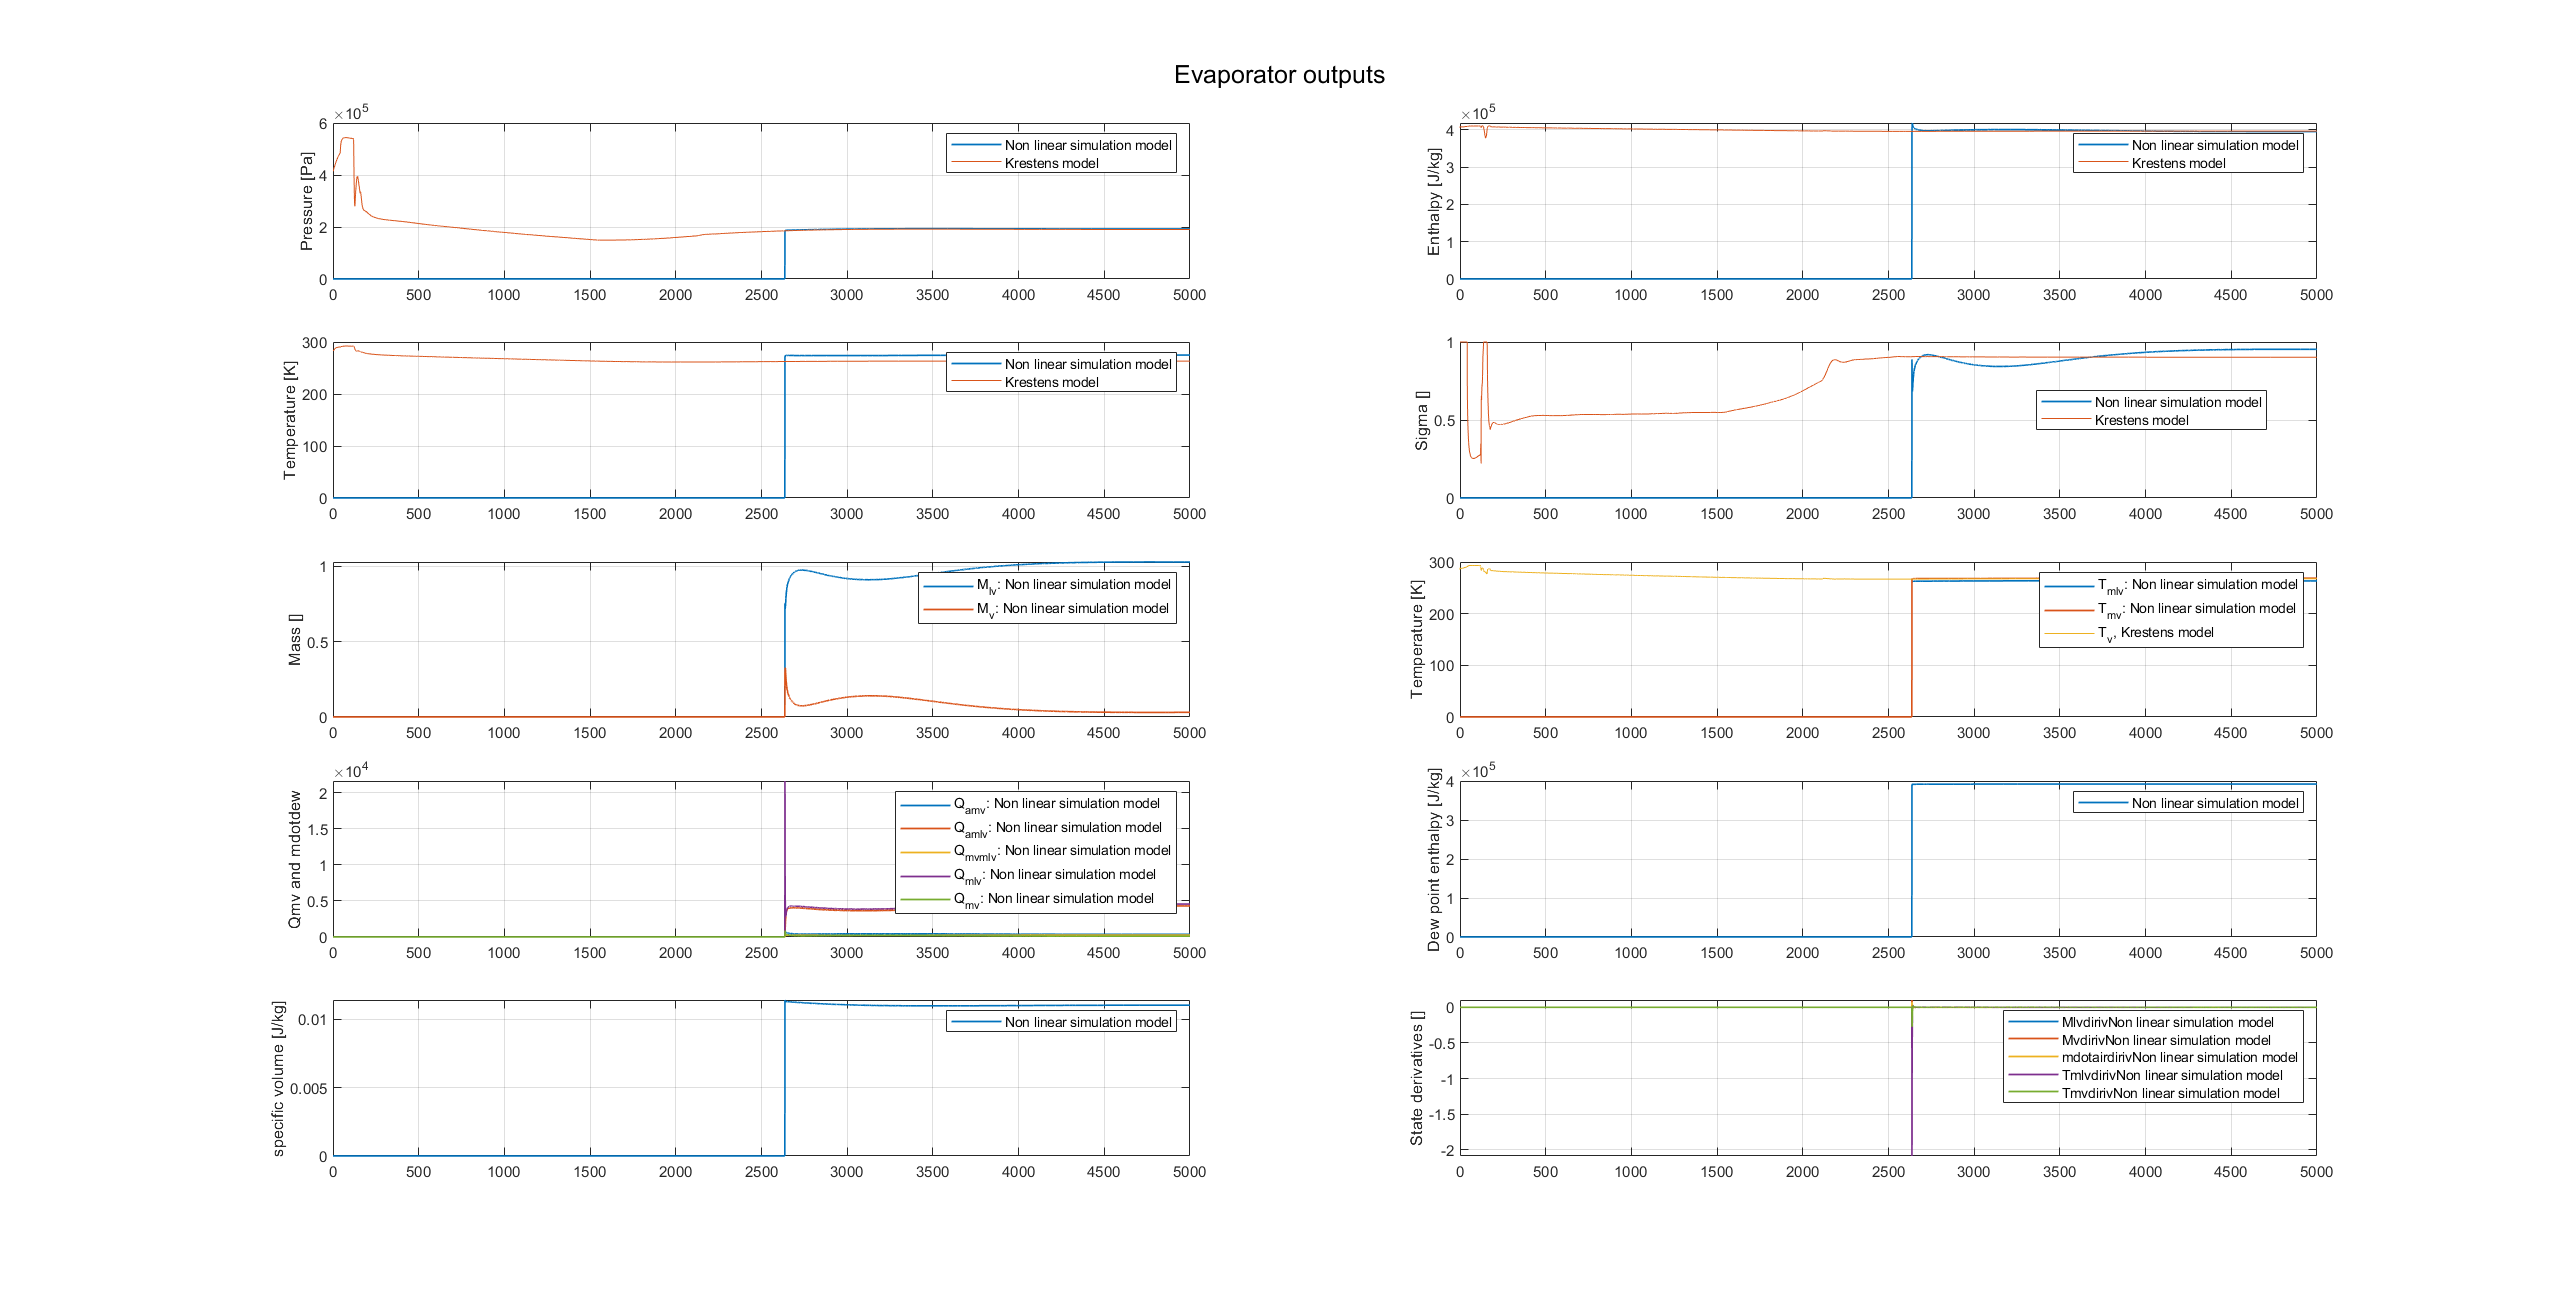
\includegraphics[width=2.1\textwidth]{Tests/Evapo_test1/plot_stable.png}
%	\caption{Simulation with $ p_{out} = p_{in} $}
%	\label{fig:evapotest_plot3}
%\end{figure}
%
%In \cref{fig:evapotest_plot3} where the output pressure is now equal to the input pressure, the behavior is much better, and for this reason we make the assumption that the output pressure is equal to the input pressure.
%
%\clearpage
\subsubsection*{Sources of error and insecurities}
